\chapter{Numerical methods used in atmospheric models}\label{ch:chapter3}
\lastupdated{2024-12-08}{\chapterThreeNumMethOverleaf}

\begin{center}
	\textit{Major content of this chapter is taken from prof.Navarra's teaching resources, available in his website \url{https://wanderer.cmcc.it/index_GARP.html}}
\end{center}
\section{Historical introduction}
In this chapter, following a short historical introduction on the development and use of numerical methods in atmospheric models, methods available for numerical solution of the differential equations governing the atmosphere will be briefly reviewed. Then, basic elements of the finite difference method for solving these equations will be introduced. Finally, the concept of stability of finite difference equations, and methods for testing the stability of such equations, will be discussed at some length.

It is considered that Wilhelm Bjerknes (1904) was the first to point out that the future state of the atmosphere can in principle be obtained by an integration of differential equations which govern the behavior of the atmosphere, using as initial values fields describing an observed state of the atmosphere. Such an integration performed using numerical methods is called \textit{numerical weather prediction}. When, however, a numerical integration is performed starting from fictitious initial fields, it is called \textit{numerical simulation}.

A first practical attempt at a numerical weather prediction was made by Richardson. After very tedious and time-consuming computations, carried out mostly during the First World War, Richardson obtained a totally unacceptable result. Despite this, he described his method and results in a book (Richardson, 1922), and this is today one of the most famous in meteorology.

The wrong result obtained by Richardson, and his estimate that 64,000 men are necessary to advance the calculations as fast as the weather itself is advancing, left some doubt as to whether the method would be of practical use. A number of developments that followed, however, improved the situation. Courant, Friedrichs and Lewy (1928) found that space and time increments in integrations of this type have to meet a certain stability criterion. Mainly due to the work of Rossby in the late 1930’s, it became understood that even a rather simple equation, that describing the conservation of absolute vorticity following the motion of air particles, suffices for an approximate description of large-scale motions of the atmosphere. Finally, in 1945, the first electronic computer ENIAC (Electronic Numerical Integrator and Computer) was constructed. The absolute vorticity conservation equation, and this first electronic computer, were used by Charney, Fjortoft and von Neumann in the late 1940’s for the first successful numerical forecast (Charney et al., 1950).

Much faster computers, and improved understanding of computational problems, now also enable long-term integrations of the basic primitive equations. It is generally considered that integration of the primitive equations enables easier incorporation of various physical processes than the integration of modified equations, that is, integration of the divergence and vorticity equations. Thus, it is mostly the primitive equations that are used today for practical numerical forecasting by meteorological services. Charts obtained by numerical forecasting are used by synopticians in these services as the principal basis for decisions on forecasts issued for public use.

A number of research groups have been actively engaged for more than a decade in development of models for the numerical simulation of the general circulation of the atmosphere. In such simulations starting from a fictitious initial state, e.g. an isothermal and motionless atmosphere, is often considered to be an advantage for the experiments. It enables a test of the ability of the computational and physical schemes of the model to simulate an atmosphere with statistical properties similar to those of the real atmosphere, with no, or not much, prior information on these properties.

Numerical models are also very frequently developed for studies of some smaller-scale atmospheric phenomena. Foremost among these are studies of the cumulus convection problem, and simulation of processes within the planetary boundary layer. In this text, however, we shall primarily have in mind the application of numerical methods to prediction and simulation of large-scale atmospheric motions.



\section{Methods for the numerical solution of the equations of motion}
Numerical solution of the equations of motion today in most cases is performed using the \textit{grid point method}. In this method a set of points is introduced in the region of interest and dependent variables are initially defined and subsequently computed at these points. This set of points is called the grid. The words mesh or lattice are also used. It is necessary to have the grid points at fixed locations in the horizontal. This means that, according to the Eulerian system of equations, space and time coordinates are chosen as independent variables.

A number of attempts have been made to develop atmospheric models using an approach which is at least partly Lagrangian\footnote{The Eulerian approach focuses on observing how a field (like fluid flow) changes at fixed points in space over time, much like watching traffic from a fixed camera. In contrast, the Lagrangian approach tracks individual elements or particles as they move through space and time, similar to following a specific car on its journey. Essentially, Eulerian examines the "big picture" from a stationary perspective, while Lagrangian follows individual components in motion.}. Serious difficulties are encountered when a straightforward numerical integration of the Lagrangian system of equations is undertaken. However, it is possible to construct methods with some Lagrangian properties; for example, to have some or all of the compu­tation points moving with the fluid. In hydrodynamics a number of such methods have proved to be very useful, especially for some problems which are not amenable to treatment by a strictly Eulerian technique (e.g. Harlow and Amsden, 1971). However, in meteorology the per­formance of Lagrangian or semi-Lagrangian models that have so far been developed has not been quite satis­factory. A discussion of one way of constructing a Lagrangian model, and a review of earlier attempts, can be found in a paper by Mesinger (1971).

Another possible approach is to express the spatial dependence of the variables in terms of a series of ortho­gonal functions, and then substitute this into the governing equations. In this way the equations reduce to a set of ordinary differential equations, so that the coefficients of the series can be computed as functions of time. This is the \textit{spectral method} of solving the governing equations. Until relatively recently it was considered that in effi­ciency the spectral method could not be competitive with the grid point method. But the use of the fast Fourier transform has completely changed the situation and investigation of spectral methods is now the subject of intensive research.

In the following we shall consider the technique of using the grid point method, and the problems associated with it, using grid of computation points fixed in space. This is the most direct way of solving the equations of motion numerically. Furthermore, knowledge of this method is necessary for the investigation and understanding of the relative merits of other alternatives mentioned in this section.
\section{Grid point method}
With the grid point method, the most common way of solving the governing equations is to find approximate expressions for derivatives appearing in the equations. These approximate expressions are defined using only values of the dependent variables at the grid points, and at discrete time intervals. Thus, they are formed using differences of dependent variables over finite space and time intervals; for that reason this approach is called the \textit{finite difference method}. The approximations for derivatives are then used to construct a system of algebraic equations that approximates the governing partial differential equations. This algebraic system is considered valid at each of the interior grid points of the computation region. For the initial time and at space boundary points, additional constraints or equa­tions are defined that approximate the initial and bound­ary conditions as required by the physics of the problem. The set of algebraic equations obtained in this way is then solved, usually using an electronic computer, by a suitable step-wise procedure.

We shall now consider some basic elements of the finite difference method. For simplicity, we start by considering a function of one independent variable $$u=u(x)$$
The function $u$ is a solution to a differential equation that we are interested in. We want to find an approxima­tion to this solution in a bounded region R of the inde­pendent variable, having a length \textit{L}. The simplest way of introducing a set of grid points is to require that they divide the region R into an integer number of intervals of equal length $\Delta x$. This length $\Delta x$ is called the \textit{grid interval}, or \textit{grid length}. Let us denote the number of grid intervals by \textit{J}. It is convenient to locate the origin of the \textit{x} axis at the left-hand end of the region R. Thus, we are looking for approximations to $u(x)$ at discrete points $x=j\Delta x$, where \textit{j} takes integer values 0,1,2,… \textit{J}. These approximate values we shall denote by $$u_j=u_j(j\Delta x)$$
Thus, we are interested in finding \textit{J} + 1 values $u_j$

Knowledge of a discrete set of values $u_j$, even if the approximations were perfect, offers, obviously, less information than knowledge of the function $u(x)$. Let us briefly consider the situation in that respect. We shall very often find it convenient to think of the function $u(x)$ as being formed by a sum of its Fourier compo­nents, that is
$$u(x)=\frac{a_0}{2}+\displaystyle\sum_{n\geq 1}[a_n\cos\big(2\pi n\frac{x}{L}\big)+b_n\sin\big(2\pi n\frac{x}{L}\big)]$$

Now, the available \textit{J} + 1 values $u_j$ do not enable the computation of all of the coefficients $a_nb_n$; rather, they can be used to compute only \textit{J} + 1 different coefficients. A natural choice is to assume that the \textit{J} + 1 values $u_j$ define the near value $a_0$ and as many as possible of the coefficients of the Fourier components at the long wave length end of the series, that is, coefficients for \textit{n} = 1,2,3,…, \textit{J/} 2. Of these components, the one with the shortest wavelength will have $n=J/2$, with the wave length
$$\frac{L}{n}=\frac{2L}{j}=\frac{2L}{\frac{L}{\Delta x}}=2\Delta x$$
Having made that choice, we can say that with values $u_j$ at discrete points $x=j\Delta x$ it is not possible to resolve waves with wave length shorter that $2\Delta x$.
Now let us consider the differences between values $u$ that will be used to construct approximations to derivatives. These differences are called \textit{finite differences}. They can be calculated over one or more of the intervals $\Delta x$. Depending on the relation of the points from which the values are taken to the point where the derivative is required, they can be \textit{centered or uncentered}. An un-centered difference is, for example, the \textit{forward} difference

\begin{equation}\label{eq: forward difference}
	\Delta u_j=u_{j+1}-u_j
\end{equation}
more often centered (or central) differences are used, such as
\begin{equation}
	\Delta u_{j+1/2}=u_{j+1}-u_j
\end{equation}
In a centered difference the difference is between values symmetrical about the point where the difference is being calculated.

One way to construct an approximation to a differential equation is to simply replace the derivatives by appropriate \textit{finite difference quotients}. For example, for the first derivative one can use the approximation (in a forward difference scheme):
\begin{equation}\label{eq.finite diff der approx}
	\left(\frac{d u}{dx}\right)_j\rightarrow\frac{u_{j+1}-u_j}{\Delta x}
\end{equation}
The finite difference quotient here is, of course, only one of many possible approximations to the first derivative at point j.

If a finite difference quotient, or a more complex expression, is to be used as an approximation to a deri­vative, it is required, above all, that this approximation be consistent. This means that the approximation should approach the derivative when the grid interval approaches zero. The quotient \ref{eq.finite diff der approx} , obviously, has that property.

Important information is obatined when the true solution $u(j\Delta x)$ is substituted into an approximation to the derivative in place of the grid point values $u_j$, and$ u(j\Delta x)$ is expanded in a Taylor series about the central point. For the quotient \ref{eq.finite diff der approx} this procedure gives
\begin{equation}
	\frac{u_{j+1}-u_j}{\Delta x}\rightarrow\left(\frac{du}{dx}\right)_j+\frac{1}{2}\left(\frac{d^2u}{dx^2}\right)_j\Delta x+\frac{1}{6}\left(\frac{d^3u}{dx^3}\right)_j(\Delta x)^2+\dots
\end{equation}
The difference between this expression and the derivative $$\left(\frac{du}{dx}\right)_j$$ being approximated. In this case:
\begin{equation}
	\epsilon= \frac{1}{2}\left(\frac{d^2u}{dx^2}\right)\Delta x+\frac{1}{6}\left(\frac{d^3u}{dx^3}\right)_j
\end{equation}
is called the \textit{truncation error} of the approximation to the derivative. These are terms that were "truncated off" to form the approximation. The truncation error gives a measure of how accurately the difference quotient approximates the derivative for small values of $\Delta x$. The usual measure of this is the order of accuracy of an approximation. This is the lowest power of $\Delta x$ that appears in the truncation error. Thus, approximation \ref{eq.finite diff der approx}
is of the first order of accuracy. We can write
\begin{equation}
	\epsilon =o(\Delta x)
\end{equation}
For an approximation to the derivative to be consistent it must, obviously, be at least first order accurate.
\subsection{Finite difference schemes}
The algebraic equation obtained when derivatives in a differential equation are replaced by appropriate finite difference approximations is called a finite difference approximation to that differential equation, or a finite difference scheme. In this section we shall introduce the concepts of consistency, truncation error, and accuracy, for a finite difference scheme.

As an example, we shall use the linear advection equation
\begin{align}\label{eq:linear adv eq}
	\frac{\partial u}{\partial t}+d\frac{\partial u}{\partial x}=0 \notag \\
	u=u(x,t)
\end{align}
$c$ is a positive constant.
It describes advection of the variable $u$ at a constant velocity $c$ in the direction of the $x$ axis. The solution to this simple equation can, of course, also be obtained by an analytic method. It will be useful to obtain the analytic solution first, in order to investigate properties of numerical solutions by comparing them against known properties of the true solution.

It is convenient to this end to change from variables $x$, $t$ to variables $\xi$ and $t$ with the substitution $\xi=x-ct$.

Using the notation
$$u^{(x,t)}=U(\xi,t)$$
we obtain:
\begin{align}
	\frac{\partial u}{\partial t}=\frac{\partial U}{\partial\xi}\frac{\partial\xi}{\partial t}+\frac{\partial U}{\partial t}\frac{\partial t}{\partial t}=-c\frac{\partial U}{\partial\xi}+\frac{\partial U}{\partial t} \\
	\frac{\partial u}{\partial x}=\frac{\partial U}{\partial\xi}\frac{\partial\xi}{\partial x}+\frac{\partial U}{\partial t}\frac{\partial t}{\partial x}=\frac{\partial U}{\partial\xi}
\end{align}
that, substitued into \ref{eq:linear adv eq}, gives
$$\frac{\partial}{\partial t}U(\xi, t)=0$$
Thus, it is seen that U cannot be a function of $t$, but can be an arbitrary function of $\xi$. A solution of \ref{eq:linear adv eq} is, therefore,
\begin{equation}\label{eq:sol of linear adv eq}
	u=f(x-ct)
\end{equation}
where $f$ is an arbitrary function. This, we see, is the general solution of the advection equation \ref{eq:linear adv eq}, since it can satisfy an arbitrary initial condition
\begin{equation}
	u(x,0)=F(x)
\end{equation}
Thus,
\begin{equation}
	u=F(x-ct)
\end{equation}
is the solution of \ref{eq:linear adv eq} satisfying the initial conditions.
For a physical interpretation, it is often convenient to consider the solution in the $x, t$ plane. In the present case, we see that the solution takes constant values along the straight lines
$$x-ct= \text{const}$$
These lines are the \textit{characteristics} of the advection equa­tion. We can say that the solution propagates along the characteristics.\\





Let us now construct a scheme for finding an approxi­mate solution to \ref{eq:linear adv eq} using the grid point method.

We are now looking only for an approximate solution at the discrete points in the $(x,t)$ plane formed by the grid shown in the figure below. The approximate solution at a point $(j\Delta x,n\Delta t)$ is denoted by $u^n_j$.
\begin{figure}[htpb]
	\centering
	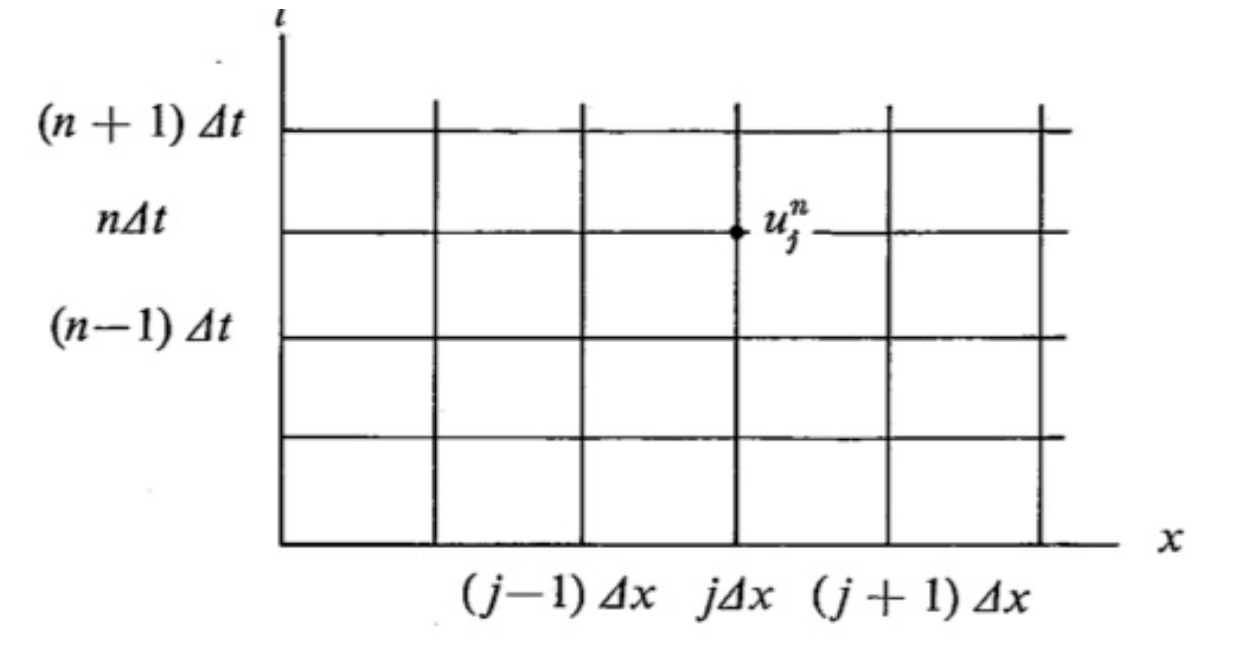
\includegraphics[width=0.35\linewidth]{uploads/Screenshot 2024-12-07 163047.png}
	\caption{A finite difference grid for finding an approximate solution of \ref{eq:linear adv eq}}
	\label{fig:grid sol lin adv eq}
\end{figure}

The behaviour of the true solution, which propagates along characteristics in the $(x,t)$ plane, suggests constructing the approximate equation by replacing the time derivative by a forward difference quotient, and the space derivative by a backward difference quotient. In this way we obtain the scheme
\begin{equation}\label{eq:forward and upward scheme}
	\frac{u_j^{n+1}-u_j^n}{\Delta t}+c\frac{u_j^n-u^n_{j-1}}{\Delta x}=0
\end{equation}

This scheme could be called a forward and upstream scheme, the latter word indicating the position of the point $j-1$ relative to the advection velocity. It is, of course, only one of many possible consistent finite difference schemes for the differential equation. There are many schemes which approach the differential equation when the increments $\Delta x,\Delta t$ approach zero.

Since for small values of $\Delta x, \Delta t$ a finite difference equation approximates the corresponding differential equation, we can expect that its solution will be an approximation to the solution of that equation. We shall call solutions given by finite difference schemes numerical solutions. There are, of course, both approximate and numerical solutions obtained by other methods which will not be considered in this publication. It is most convenient to study the properties of numerical solutions when they can be compared with known solutions of the original differential equation, which we shall refer to as true solutions. The difference between the numerical and the true solution
\begin{equation}
	u_j^n-u(j\Delta x,n\Delta t)
\end{equation}
is the error of the numerical solution. For obvious reasons, we cannot often expect to know the error of the numerical solution. However, we can always find a measure of the accuracy of the scheme by substituting the true solution $u(j\Delta x, n\Delta t)$ of the equation, into the numerical scheme. Since the true solution will not satisfy the numerical equations exactly, we will have to add an additional term to keep the equation valid. Let us denote this term by $\epsilon$. For example, in the case of scheme \ref{eq:forward and upward scheme} this procedure gives
\begin{equation}\label{eq:2.4.7}
	\frac{u(j\Delta x,(n+1)\Delta t)-u(j\Delta x, n\Delta t)}{\Delta t}+c\frac{u(j\Delta x, n\Delta t)-u((j-1\Delta x, \Delta t)}{\Delta x}=\epsilon
\end{equation}
The term $\epsilon$ we shall call the truncation error of the finite difference scheme. It shows how closely the true solution satisfies the equation of the scheme, and, thus, gives a measure of the accuracy of the scheme.

We can obtain a more useful form for the expression for the truncation error by performing a Taylor series expansion of the true solution about the central space and time point. Using the original differential equation to eliminate the leading term we obtain the truncation error \ref{eq:2.4.7}:
\begin{equation}\label{eq: 2.4.8}
	\epsilon=\frac{1}{2}\frac{\partial^2u}{\partial t^2}\Delta t+\frac{1}{6}\frac{\partial^3u}{\partial t^3}(\Delta t)^2+\dots-c\left(\frac{1}{2}\frac{\partial^2u}{\partial x^2}\Delta x-\frac{1}{6}\frac{\partial^3u}{\partial t^3}(\Delta x)^2+\dots\right)
\end{equation}
As before, these are the terms that were “truncated off” to make the differential equation reduce to our finite difference scheme.

In the same way as for an approximation to the derivative, the order of accuracy of a finite difference scheme is the lowest power of $\Delta x$ and $\Delta t$ that appears in the truncation error. Thus, scheme \ref{eq:forward and upward scheme} is first order accurate. We can write
$$\epsilon=o(\Delta t)+o(\Delta x)=o(\Delta x,\Delta t)$$
It is useful to make a distinction between orders of accuracy in space and in time, especially when the lowest powers of $\Delta x$ and $\Delta t$ are not the same. As before, a necessary condition for consistency of a scheme is that it be at least of the first order of accuracy.
\subsection{Convergence}
The truncation error of a consistent scheme can be made arbitrarily small by a sufficient reduction of the increments $\Delta x$ and $\Delta t$. Unfortunately, we cannot be sure that this will also result in a reduction of the error of the numerical solution. For that reason, we return to consideration of the error
$$u_j^n-u(j\Delta x,n\Delta t)$$
Following Richtmyer and Morton (1967) we ask two questions:
\begin{itemize}
	\item What us the bahaviour of the error $u_j^n-u(j\Delta x, n\Delta t)$ when, for a fixed total time $n\Delta t$ the increments $\Delta x, \Delta t$ approach zero?
	\item What is the behaviour of the error $u_j^n-u(j\Delta x, n\Delta t)$ when, for fixed values of $\Delta x, \Delta t$, the number of time steps $n$ increases?
\end{itemize}

The answer to the first of these questions depends on the convergence of the numerical solution: if the error approaches zero as the grid is refined (as $\Delta x\Delta t\rightarrow 0$) the solution is called convergent. If a scheme gives a convergent solution for any initial conditions, then the scheme also is called convergent.

Consistency of a scheme does not guarantee convergence. We shall illustrate this by a simple example. We still consider the scheme \ref{eq:forward and upward scheme}; its truncation error \ref{eq: 2.4.8} approaches zero as the grid is refined, and, therefore, this is a consistent scheme. But consider the numerical solution, when the grid lines and characteristics are as shown in the figure below. The characteristic passing through the grid point taken as the origin in this example passes through another grid point, A, denoted by a square. Thus, the true solution at A, is equal to the initial value at the origin. However the numerical solution given by \ref{eq:forward and upward scheme} A is computed using the values at points denoted by circles. The shaded domain, including all of these points, is called \textit{the domain of dependence} of the numerical scheme. The grid point at the origin is outside that domain, and, thus, cannot affect the numerical solution at $A_0$. Therefore, the error can be arbitrarily great. If the space and time steps were reduced by the same relative amount, say to one half of their values in the figure, the domain of dependence would still remain the same, and this situation would not change. Thus, as long as the ratio of the steps $\Delta x$ and $\Delta t$ remains the same, refinement of the grid cannot bring about a reduction in the error of the numerical solution.
$$x-ct=\text{const}$$
A necessary condition for convergence of a scheme is, obviously, that the characteristic defining the true solution at a grid point is inside the domain of dependence of the numerical solution at that point. In our example, this will happen when the slope of the characteristics is greater than the slope of the dashed line bounding the domain of dependence, that is, when $$c\Delta t\leq \Delta x$$
thus, this is a necessary condition for convergence of \ref{eq:forward and upward scheme}
\begin{figure}[h]
	\centering
	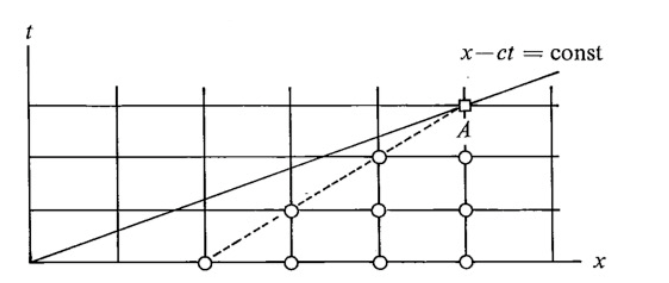
\includegraphics[width=7cm]{uploads/Screenshot 2024-11-10 192132.png}
	\caption{A possible relative position of a characteristic and of a domain of dependence}
	\label{fig:grid sol}
\end{figure}
\subsection{Stability}
The answer to the second question raised at the beginning of the section Convergence "What is the behaviour of the error $u_j^n-u(j\Delta x, n\Delta t)$ when, for fixed values of $\Delta x, \Delta t$, the number of time steps $n$ increases?" depends on the stability of the numerical solution. A rigorous definition fo stability employs the concepts of functional analysis, and refers to the boundedness of the numerical solution only (e.g. Richtmyer and Morton, 1967). The difficulties in defining stability are caused by the fact that the true solution, in general, does not have to be bounded. However, when we know that the true solution is bounded, as in the equations we are interested in here, we can use a definition referring to the boundedness of the error $u_j^n-u(j\Delta x, n\Delta t)$. We said that a solution $u_j^n$ is stable if this error remains bounded as $n$ increases, for fixed values of $\Delta x, \Delta t$. As before, we say that \textbf{a finite difference scheme is stable if it gives a stable solution for any initial condition}.

Stability of a scheme is a property of great practical significance. There are consistent schemes, of a high order of accuracy, that still give solutions diverging unacceptably fast from the true solution. Thus, conditions for stability, if any, should be known. There are three methods that can be used to investigate the stability of a scheme, and we shall give an example of each of these methods. We shall do this by considering again the forward and upstream scheme \ref{eq:forward and upward scheme}.


\textcolor{Blue}{\textit{Direct method}} tests mathematically the stability of a scheme. Since we know that the true solution is bounded, it suffices to test the boundedness of the numerical solution. The scheme \ref{eq:forward and upward scheme} can be written as
\begin{equation}\label{2.6.1}
	u_j^{n+1}=(1+\mu)u_j^n+\mu u^n_{j-1}
\end{equation}
where
$$\mu=c\frac{\Delta t}{\Delta x}$$
if $1-\mu\geq 0$, which happens to be also the necessary condition for convergence, we will have:
\begin{equation}\label{2.6.2}
	|\mu_j^{n+1}|\leq(1-\mu)|u_j^n|+\mu|u^n_{j-1}|
\end{equation}
We can apply this at the point where at time level $n+1$, $|u_j^{n+1}|$ is a maximum, $Max_{(j)}|u_j^{n+1}|$. The right side of \ref{2.6.2} can only be increased by replacing $|u_j^n$ and $|u_{j-1}^n|$ by the maximum value at level $n$, $Max_{(j)}|u_j^n|$. The two terms on the right side can be added, and we obtain
$$Max_{(j)}|u_j^{n+1}|\leq Max_{(j)}|u_j^n|$$
This proves the boundedness of the numerical solution. Hence, $1-\mu\geq 0$ is seen to be a sufficient condition for stability of \ref{2.6.1}.

This direct testing of the stability is simple. Unfortunately, as might be anticipated from the argument, it is successful only for a rather limited number of schemes.\\



\textcolor{Blue}{\textit{Energy method}}. This method is of a much wider applicability, and can be used even for nonlinear equations. If we know that the true solution is bounded, we test whether
$$\displaystyle\sum_j(u_j^n)^2$$
is also bounded.
If it is, then every value \(u_j^n\) must be bounded, and the stability of the scheme has been proved. The method is called the energy method since in physical applications \(u^2\) is often proportional to some form of energy. Of course, there are examples when this is not so.
\begin{figure}[htpb]
	\centering
	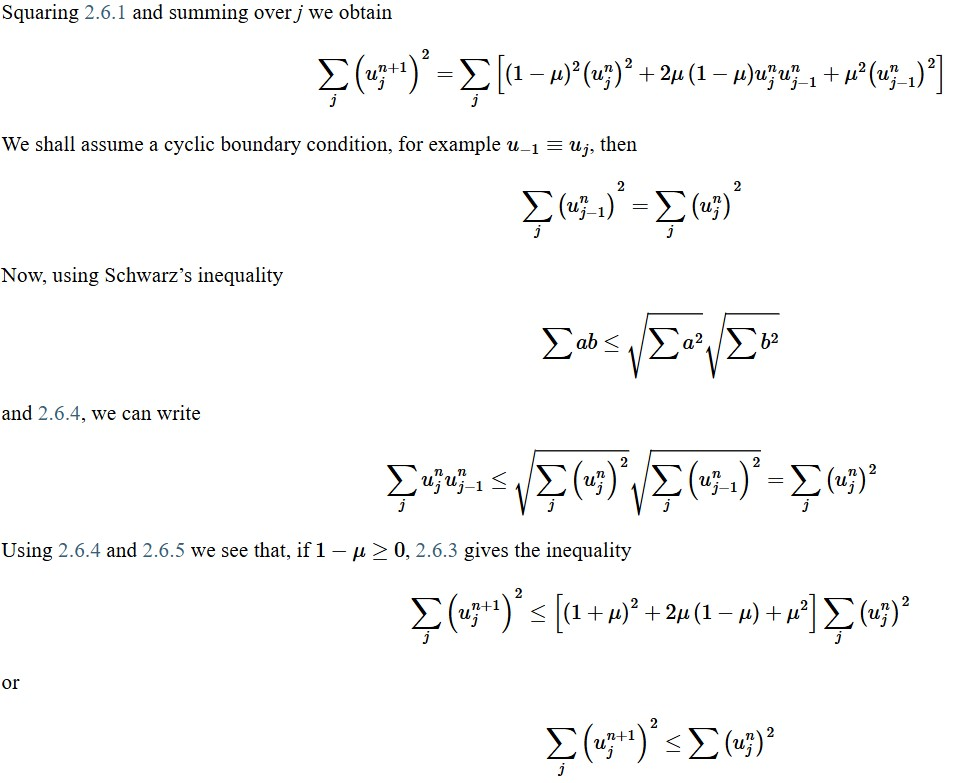
\includegraphics[width=0.75\linewidth]{uploads/Immagine 2024-12-07 101350.jpg}
\end{figure}
\textit{ Von Neumann’s,} or the Fourier series method is the most frequently used method of linear equations that can be expressed in form of a Fourier series, where each harmonic component is also a solution. Thus, we can test the stability of a single harmonic solution ; stability of all admissible harmonics will then be a necessary condition for stability of the scheme.
%For an illustration of this method, it is useful first to obtain an analytic solution of the advection equation :
\begin{figure}[htpb]
	\centering
	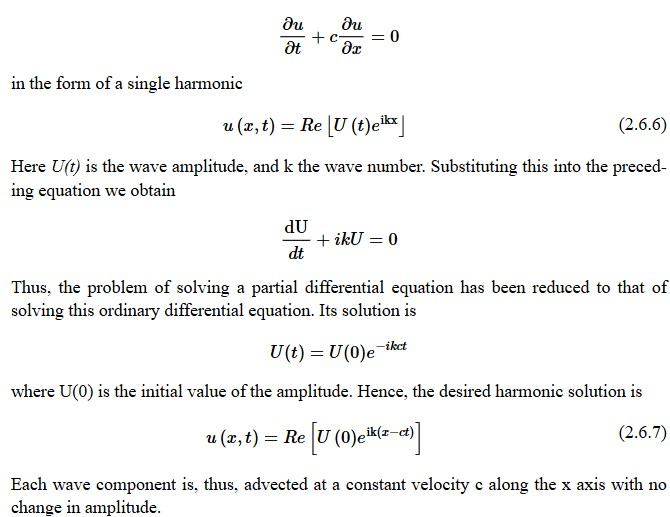
\includegraphics[width=0.70\linewidth]{uploads/Immagine 2024-12-07 102403.jpg}
\end{figure}
A harmonic  solution of the finite difference advection equation.
\begin{figure}[htp!]
	\centering
	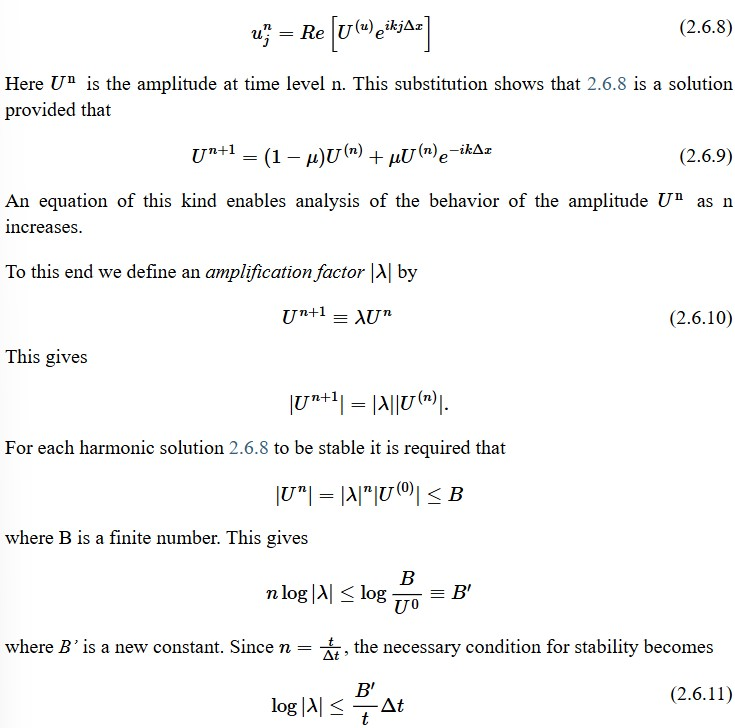
\includegraphics[width=0.65\linewidth]{uploads/Immagine 2024-12-07 103148.jpg}
\end{figure}
\begin{figure}[htp!]
	\centering
	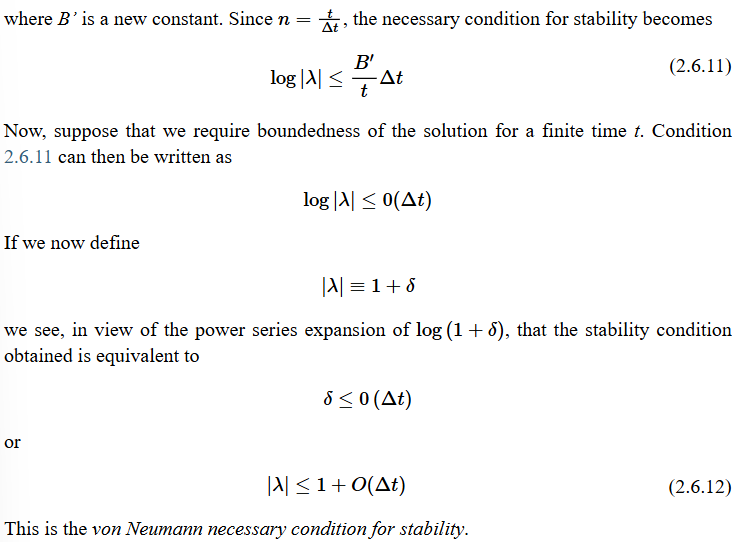
\includegraphics[width=0.65\linewidth]{uploads/hhhhh.png}
\end{figure}

The Von Neumann condition permits exponential growth of the solution, but no faster. This is useful for analyzing cases where the true solution grows exponentially. However, when the true solution does not grow, as in example 2.6.7, it is common to replace the von Neumann condition with a sufficient condition, much less generous than that required by the original definition of stability : \(|\lambda|\leq1\).
\begin{figure}[htp!]
	\centering
	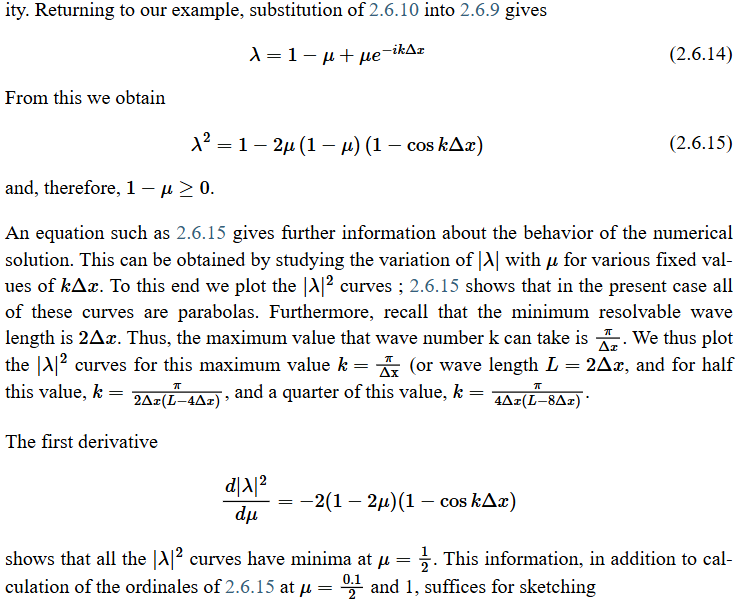
\includegraphics[width=0.65\linewidth]{uploads/mi.png}
\end{figure}
\begin{figure}[htpb]
	\centering
	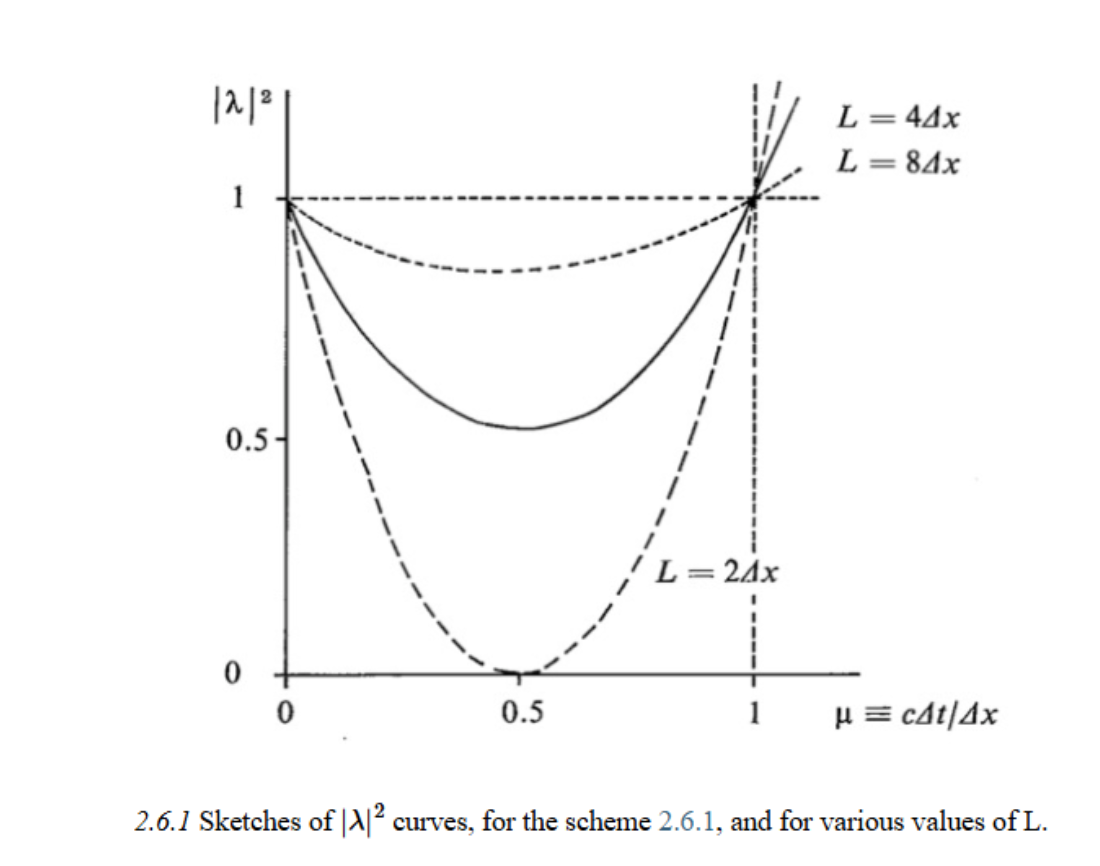
\includegraphics[width=0.45\linewidth]{uploads/pp.png}
\end{figure}

The graphs of the $|\lambda|^2$ curves are shown in the picture above. In general, as the wave length $L$ increases, that is, as $k$ approaches to zero, the amplification factor approaches unity for any value of the parameter $\mu$. The figure shows that within the stable region the scheme is damping for all values $\mu\leq 1$. The damping increases as the wave length decreases. Since the true solution has a constant amplitude, this damping reveals an error due to finite differencing. We can see that this error increases as the wave length decreases. At the shortest resolvable wave length $L=2\Delta x$, the error may be very great unless $\Delta t$ extremely small. It is even possible for this wave to be completely removed after only a single time step.


The error's dependence on wavelength can be understood by considering how the finite difference grid represents harmonics of different wavelengths. The shortest resolvable wave, with only two data points per wavelength, is poorly represented. As the wavelength increases, the representation improves and approaches the continuous representation as the wavelength tends to infinity.



\section{Time differencing schemes}
In this chapter we consider ordinary differential equations with one dependent and one independent variable. Although atmospheric models are essentially always models for solving a complex set of partial differential equations, in some formulations the numerical solution of ordinary differential equations forms an important part of the computational procedure. For instance in spectral models the governing partial differential equations reduce to a set of ordinary differential equations for the expansion coefficients as dependent variables. A set of ordinary differential equations will also be obtained if a Lagrangian method is used, in which the computational points move with the fluid. But, most of all, schemes for solving ordinary differential equations are of interest here since they are often used without modification to construct approximations to the time derivative terms in the governing partial differential equations. Knowledge of the properties of schemes for solving ordinary differential equations will then be used in investigating the properties of more complex schemes for solving the partial differential equations.

With that in mind, we shall here first define some of the schemes that will be interesting to analyze. Then we shall investigate the behavior of numerical solutions obtained when these schemes are used for two specific ordinary differential equations: the oscillation (or frequency) equation, and the friction equation. These equations will serve as prototypes for later extension of the results to advection, gravity-inertia wave, and diffusion processes within the atmospheric primitive equations.

Schemes used for the time derivative terms within the primitive equations are relatively simple, usually of the second and sometimes even only of the first order of accuracy. There are several reasons for this. First, it is a general experience that schemes constructed so as to have a high order of accuracy are mostly not very successful when solving partial differential equations. This is in contrast to the experience with ordinary differential equations, where very accurate schemes, such as the Runge-Kutta method, are extremely rewarding. There is a basic reason for this difference. With an ordinary differential equation, the equation and a single initial condition is all that is required for an exact solution. Thus, the error of the numerical solution is entirely due to the inadequacy of the scheme. With a partial differential equation, the error of the numerical solution is brought about both by the inadequacy of the scheme and by insufficient information about the initial conditions, since they are known only at discrete space points. Thus, an increase in the accuracy of the scheme improves only one of these two components, and the results are not too impressive.

Another reason for not requiring a scheme of high accuracy for approximations to the time derivative terms is that, in order to meet a stability requirement of the type discussed in the preceding sections, it is usually necessary to choose a time step significantly smaller than that required for adequate accuracy. With the time step usually chosen, other errors, for example in the space differencing, are much greater than those due to the time differencing. Thus, computational effort is better spent in reducing these other errors, and not in increasing the accuracy of the time differencing. This, of course, does not mean that it is not necessary to consider carefully the properties of various possible time differencing schemes. Accuracy, is only one important consideration in choosing a scheme.

To define some schemes, we consider the equation
\begin{equation}\label{eq.3.1.3}
	\frac{dU}{dt}= f(U,t) \,\, U=U(t)
\end{equation}
We divide the time axis into segments of equal length $\Delta t$. We shall denote by
$U^{(n)}$ the approximate value of U at time $n\Delta t$. We assume that we know at least the first of the values $U^{(n)}$, $U^{(n-1)}$, $\dots$ and we want to construct a scheme for computation of an approximate value $U^{(n+1)}$. These are many possibilities.
\subsubsection{Two-level schemes}
These are schemes that relate values of the dependent variable at two time levels: $n$ and $n + 1$. Only a two level scheme can be used to advance an integration over the first time step, when just a single initial condition is available. With such a scheme we want to approximate the exact formula
\begin{equation}\label{eq. 3.1.4}
	U^{(n+1)}=U^{(n)}+\int_{n\Delta t}^{(n+1)\Delta t}f(U,t)dt
\end{equation}
Schemes that don't use an iterative procedure:
\paragraph{Euler (forward) scheme}
This is the scheme
\begin{equation}\label{3.1.5}
	U^{n+1}=U^{(n)}+\Delta t\cdot f^{(n)}
\end{equation}
where
$$f^{(n)}=f\left(U^{(n)},n\Delta t\right)$$
The truncation error of this scheme is $o(\Delta t)$. Thus, this is a first order accurate scheme. For the integrand in \ref{eq. 3.1.4} we have here taken a constant value equal to that at the lower boundary of the time interval. Thus, this is an uncentered scheme.
\paragraph{Backward scheme}
We can also take a constant value of $f$ equal to that at the upper boundary of the time interval. We then obtain
\begin{equation}\label{3.1.6}
	U^{n+1}=U^{(n)}+\Delta t f^{(n+1)}
\end{equation}

If, as here, a value of $f$ depending on $U^{(n+1)}$ appears in the difference equation, the scheme is called implicit. For an ordinary differential equation, it may be simple to solve such a difference equation for the desired value $U^{(n+1)}$. But, for partial differential equations, this will require solving a set of simultaneous equations, with one equation for each of the grid points of the computation region. If a value of $f$ depending on $U^{(n+1)}$ does not appear in the difference equation the scheme is called explicit. The truncation error of this scheme is also is $o(\Delta t)$.
\paragraph{Trapezoidal scheme}
If we approximate $f$ in \ref{eq. 3.1.4} by an average of the values at the beginning and the end of the time interval, we obtain the trapezoidal scheme:
\begin{equation}\label{3.1.7}
	U^{(n+1)}=U^{(n)}+\frac{1}{2}\Delta t\left(f^{(n)}+f^{(n+1)}\right)
\end{equation}
This is also an implicit scheme. Its truncation error, however, is $o(\Delta t^2)$. To increase the accuracy or for other reasons we can also construct iterative schemes. Two level schemes that we will now define are constructed in the same way except an iterative procedure is used to make them explicit.
\paragraph{Matsuno (or Euler-backward) scheme}
With this scheme a step is made first using the Euler scheme; the value of U obtained for time level $n+1$ is then used for an approximation to $f^{n+1}$, and this approximate value $f^{(n+1)}$ is used to make a backward step. Thus,
\begin{align}\label{3.1.8}
	U^{*(n+1)}=U^{(n)}+\Delta tf^{(n)} \\
	U^{n+1}=U^{(n)}+\Delta  tf^{*(n+1)}\notag
\end{align}
where
$$f^{*(n+1)}=f\left(U^{*(n+1)}, (n+1)\Delta t\right)$$
this is an explicit scheme, of the first order of accuracy.
\paragraph{Heun scheme}
An approximation of the trapezoidal scheme. Thus,
\begin{align}
	U^{*(n+1)}=U^{(n)}+\Delta t f^{(n)} \\
	U^{(n+1)}=U^{(n)}+\frac{1}{2}\Delta t \left(f^{(n)}+f^{*(n+1}\right) \notag
\end{align}
Thus, this is also an explicit scheme. It is of the second order of accuracy.
\subsubsection{Three level schemes}
Except at the first step, one can store the value $U^{(n-1)}$, and construct schemes taking advantage of this additional information. These are three level schemes. They may approximate the formula
\begin{equation}\label{3.1.10}
	U^{(n+1)}=U^{(n-1)}+\int_{(n-1)\Delta t}^{(n+1)\Delta t}f(U,t)dt
\end{equation}
or, they can use the additional value $U^{(n-1)}$ to make a better approximation to $f$ in \ref{eq. 3.1.4}.
\paragraph{Leapfrog scheme}
The simplest way of making a centered evaluation of the integral in \ref{3.1.10} is to take for $f$ a constant value equal to that at the middle of the interval $2\Delta t$. This gives the leapfrog scheme
\begin{equation}\label{3.1.11}
	U^{(n+1)}=U^{(n-1)}+2\Delta t\cdot f^{(n)}
\end{equation}
Its truncation error is $o(\Delta t^2)$. This is probably the scheme most widely used at present in atmospheric models. It has also been called the "mid-point rule", or "step-over" scheme.
\paragraph{Adams-Bashforth scheme}
The scheme that is usually called the Adams-Bashforth scheme in the atmospheric sciences is, in fact, a simplified version of the original Adams-Bashforth scheme, which is of the fourth order of accuracy. The simplified version is obtained when
in \ref{eq. 3.1.4} is approximated by a value obtained at the centre of the interval $\Delta t$ by a linear extrapolation using values $f^{(n-1)}$ and $f^{(n)}$. This gives
\begin{equation}\label{3.1.12}
	U^{(n+1)}=U^{(n)}+\Delta t\left(\frac{3}{2}f^{(n)}-\frac{1}{2}f^{(n-1)}\right)
\end{equation}
This also is a second order accurate scheme.
There are many other possibilities. For examples, one can approximate the integral \ref{3.1.10} using Simpson's rule, that is, by fitting a parabola to the values $f^{(n-1)}$, $f^{(n)}$ and $f^{(n+1)}$.
The implicit scheme obtained in this way is called the Milne-Simpson scheme. To illustrate the wealth of possible alternatives we note that in a paper by Young (1968) properties of 13 different schemes have been studied. Furthermore, when we are solving a more complicated partial differential equation, or a system of such equations, time (or space-time) differencing schemes can be constructed which are more complex than those which can be defined using the simple equation \ref{eq.3.1.3}. Such schemes are widely used in atmospheric models, and some of them will be described in later chapters of this publication.


\subsection{Properties of schemes applied to particular equations}
\paragraph{The advective equation} $$\frac{\partial u}{\partial t}+c\frac{\partial u}{\partial x}=0$$
has a wave solution $u(x,t)=Re[U(t)e^{ikx}]$ provided that
$$\frac{dU}{dt}+ikc=0$$
this ordinary differential equation reduces to \ref{3.2.1} if we substitute $\omega=-kc$.
The general solution of \ref{3.2.1} is
$$U(t)=U(0)e^{i\omega t}$$
or, for discrete values $t=n\Delta t$:
\begin{equation}
	U(n\Delta t)=U(0)e^{in\omega\Delta t}
\end{equation}
Thus, considering the solution in a complex plane, its argument rotates by $\omega\Delta t$ in each time step and $\Delta t$ there is no change in amplitude.

The properties of various schemes when applied to \ref{3.2.1} are conveniently analyzed using the von Neumann method. This method, as we have seen, involves defining a variable $\lambda$ by
\begin{equation}\label{3.2.3}
	U^{(n+1)}=\lambda U^{(n)}
\end{equation}
with
$$\lambda=|\lambda|e^{i\theta}$$
so
\begin{equation}\label{3.2.5}
	U^{(n)}=|\lambda|U^{(0)}e^{in\theta}
\end{equation}
with $\theta$ representing the change in argument (or phase change) of the numerical solution in each time step. Since we know that the amplitude of the true solution does not change, we shall require $|\lambda|\leq 1$ for stability.
\begin{figure}[h]
	\centering
	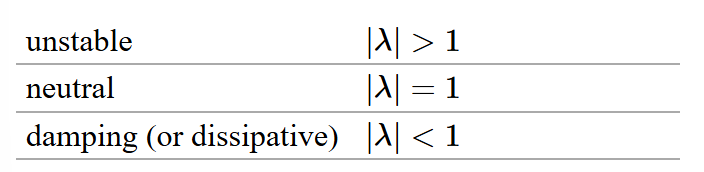
\includegraphics[width=0.50\linewidth]{uploads/Screenshot 2024-11-11 225800.png}
	\caption{stability scheme}
	\label{fig:stab scheme}
\end{figure}
It will also be instructive to compare the phase change of the numerical solution per time step, $\theta$, with that of the true solution, $\omega\Delta t$. The ratio of these changes, $\frac{\theta}{\omega\Delta t}$, is the relative phase change of the numerical solution.
\begin{figure}[h]
	\centering
	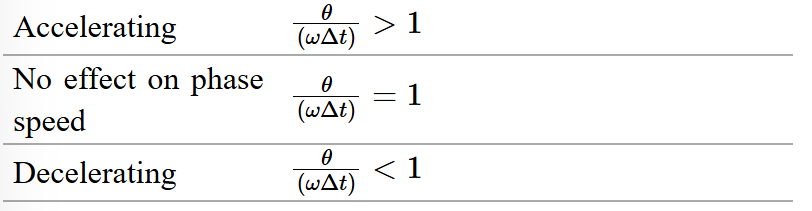
\includegraphics[width=0.50\linewidth]{uploads/Screenshot 2024-11-11 230012.png}
	\caption{phase change}
	\label{fig:phase change}
\end{figure}
For accuracy, therefore, it is desirable to have both the amplification factor and the relative phase speed close to unity. Exceptions to this are so-called “computational modes”, which, as we shall see later, can appear as false solutions superposed on the physical solution. These are solutions that do not approach the true solution as the space and time steps approach zero. If such solutions exist they will each have their own value of the amplification factor. Since they are not an approximation to the true solution, it is desirable to have their amplitudes as small as possible, that is, to have their amplification factors less than unity.\\


Stability will require, where B is a constant
\begin{equation}
	|U^{(n)}|=|\lambda|^n|U^{(0)}|<B
\end{equation}
or
\begin{equation}
	n\log|\lambda|<\log\frac{B}{|U^{(0)}|}
\end{equation}
$$\log|\lambda|<\log\frac{B\Delta t}{t|U^{(0)}|}\propto \frac{B'}{t}\Delta t$$
we want however that it is valid for finite times
$$\log|\lambda|\leq o(\Delta t)$$
This means that if $\lambda=\+\delta$ the deviation must be such that $\delta\leq o(\Delta t)$ so the condition for stability is:
\begin{equation}
	|\lambda|\leq 1+o(\Delta t)
\end{equation}
this condition will allow for exponential growth, but not faster.
\paragraph{Generale formula}
The three non-iterative two level schemes can be describes by a single finite difference equation:
\begin{equation}\label{3.2.6}
	U^{(n+1)}=U^{(n)}+\Delta t\left(\alpha f^n+\beta f^{(n+1)}\right)
\end{equation}
with a consistency requirement
$$\alpha+\beta=1$$
Notice:
\begin{itemize}
	\item $\alpha=1$, $\beta =1$ for the Euler scheme
	\item $\alpha=0$, $\beta=1$ for the backward scheme
	\item $\alpha=1/2$, $\beta=1/2$ for the trapezoidal scheme
\end{itemize}
\paragraph{Oscillation equation}
For applications in atmospheric models it is of particular interest to consider the case where $$f=i\omega U$$
Model problem:
\begin{equation}\label{3.2.1}
	\frac{dU}{dt}=i\omega U
\end{equation}
$$U^{(n)}\rightarrow U(n\Delta t)$$
The equation \ref{3.2.1} is known as the oscillation equation or frequency equation. Allowing U to be complex, \ref{3.2.1} can be thought of a representing a system of two equations. The parameter $\omega$ is real, and called the frequency.
Applying \ref{3.2.3} to the oscillation equation gives
\begin{equation}
	U^{(n+1)}=U^{(n)}+i\omega\Delta t\left(\alpha U^n+\beta U^{(n+1)}\right)
\end{equation}
In order to evaluate $\lambda$ we must solve this equation for $U^{(n+1)}$. Denoting $p=\omega\Delta t$:
\begin{equation}\label{3.2.9}
	U^{(n+1)}=\frac{1+i\alpha p}{1-i\beta p}U^{(n)}
\end{equation}
Therefore
\begin{equation}\label{3.2.10}
	\lambda=\frac{1+\alpha p}{1-i\beta p}
\end{equation}
\paragraph{Euler} $\alpha=1 \, \beta=0 \, \lambda=1+ip$
so $$|\lambda|=(1+p^2)^{1/2}$$
Te Euler scheme is always unstable, however for very small time steps $\Delta t$ $p$ is so small that
$$|\lambda|\approx 1+\frac{1}{2}p^2$$
The less restrictive von Neumann criterion is satisfied. However, experience shows that an indiscriminate use of the Euler scheme for solution of the atmospheric equations leads to amplification at a quite unacceptable rate.
\paragraph{Backward} $\alpha=0 \, \beta=1 \, \lambda=\frac{1}{1+p^2}1+ip$
so $$|\lambda|=(1+p^2)^{-1/2}$$
Te backward scheme is always stable (no matter what $\Delta t$), however is also dumping, meaning it's reducing the amplitude of the solution. The amount of damping increases as the frequency $\omega$ increases. This is often considered to be a desirable property of a scheme. For instance, we can think of a system in which a number of frequencies are present at the same time; for example, solving a system of equations of the type \ref{3.2.1}. This situation is similar to that existing in the real atmosphere. It would appear to be necessary to maintain the amplitudes of motions of different frequencies in the correct ratio. However, in numerical integrations, high frequency motions are often excited to unrealistically large amplitudes through errors in the initial data. It may then be desirable to reduce the amplitudes of high frequency motions by a selective damping in the time differencing scheme. In other words, a scheme with frequency dependent damping properties can be used to filter out undesirable high frequency motions.
\paragraph{Trapezoidal} $\alpha=1/2 \quad \beta=1/2 \quad \lambda=\frac{1}{1+1/4p^2}\left(1-1/4p^2+ip\right)$
$$|\lambda|=1$$
The trapezoidal scheme is, thus, always neutral. The amplitude of the numerical solution remains constant, just as does that of the true solution. It is useful to note that both the implicit schemes considered here were stable no matter how large a value of $\Delta t$ was chosen.
\paragraph{Matsuno}
The iterative two level schemes can also be described by a single equation in the same way as \ref{3.2.6}. Thus, we write
\begin{align}\label{3.2.18}
	U^{(n+1)*}=U^{(n)}+\Delta tf^{(n)}\notag \\
	U^{(n+1)}=U^{(n)}+\Delta t\left(\alpha f^{(n)}+\beta f^{*(n+1)}\right)
\end{align}
that applied to the oscillation equation gives:
\begin{align}
	U^{(n+1)*}=U^{(n)}+i\omega\Delta tU^{(n)} \notag \\
	U^{(n+1)}=U^{(n)}+i\omega\Delta tU^{*(n+1)}
\end{align}
eliminating the intermediate values $U^{(n+1)*}$:
$$U^{(n+1)}=\left(1-\beta p^2+ip\right)U^{(n)}$$
thus,
\begin{equation}\label{3.2.20}
	\lambda=1-\beta p^2+ip
\end{equation}
Substituting the appropriate values of $\beta$ for the Matsuno scheme, we obtain
\begin{equation}\label{3.2.21}
	\lambda=1-p^2+ip
\end{equation}
and the stability condition (we need to evaluate $|\lambda|$):
\begin{equation}\label{3.2.23}
	|\lambda|=\left(1-p^2+p^4\right)^{1/2}
\end{equation}
the Matsuno scheme is stable if $|p|<1$, so the time step must be $$\Delta t\leq\frac{1}{|\omega|}$$
This scheme is conditionally stable: the higher the frequency, the more restrictive is the stability condition. When differenciating \ref{3.2.23} we find that the amplification factor of the Matsuno scheme has a minimum for $p=1/\sqrt{2}$. Therefore, as pointed out by Matsuno (1966a) when dealing with a system with a number of frequencies we can choose a time step so as to have $0\leq p\leq 1/\sqrt{2}$ for all the frequencies present, and then, in the same way as backward implicit scheme, this scheme will reduce the relative amplitudes of high frequencies. This technique has recently become very popular for initialization of atmospheric models, where it is used to damp the spurious high frequency noise generated by the assimilation of the observed data. As shown by Matsuno (1966b) higher order accuracy schemes with similar filtering characteristics can be constructed.
\begin{figure}[h]
	\centering
	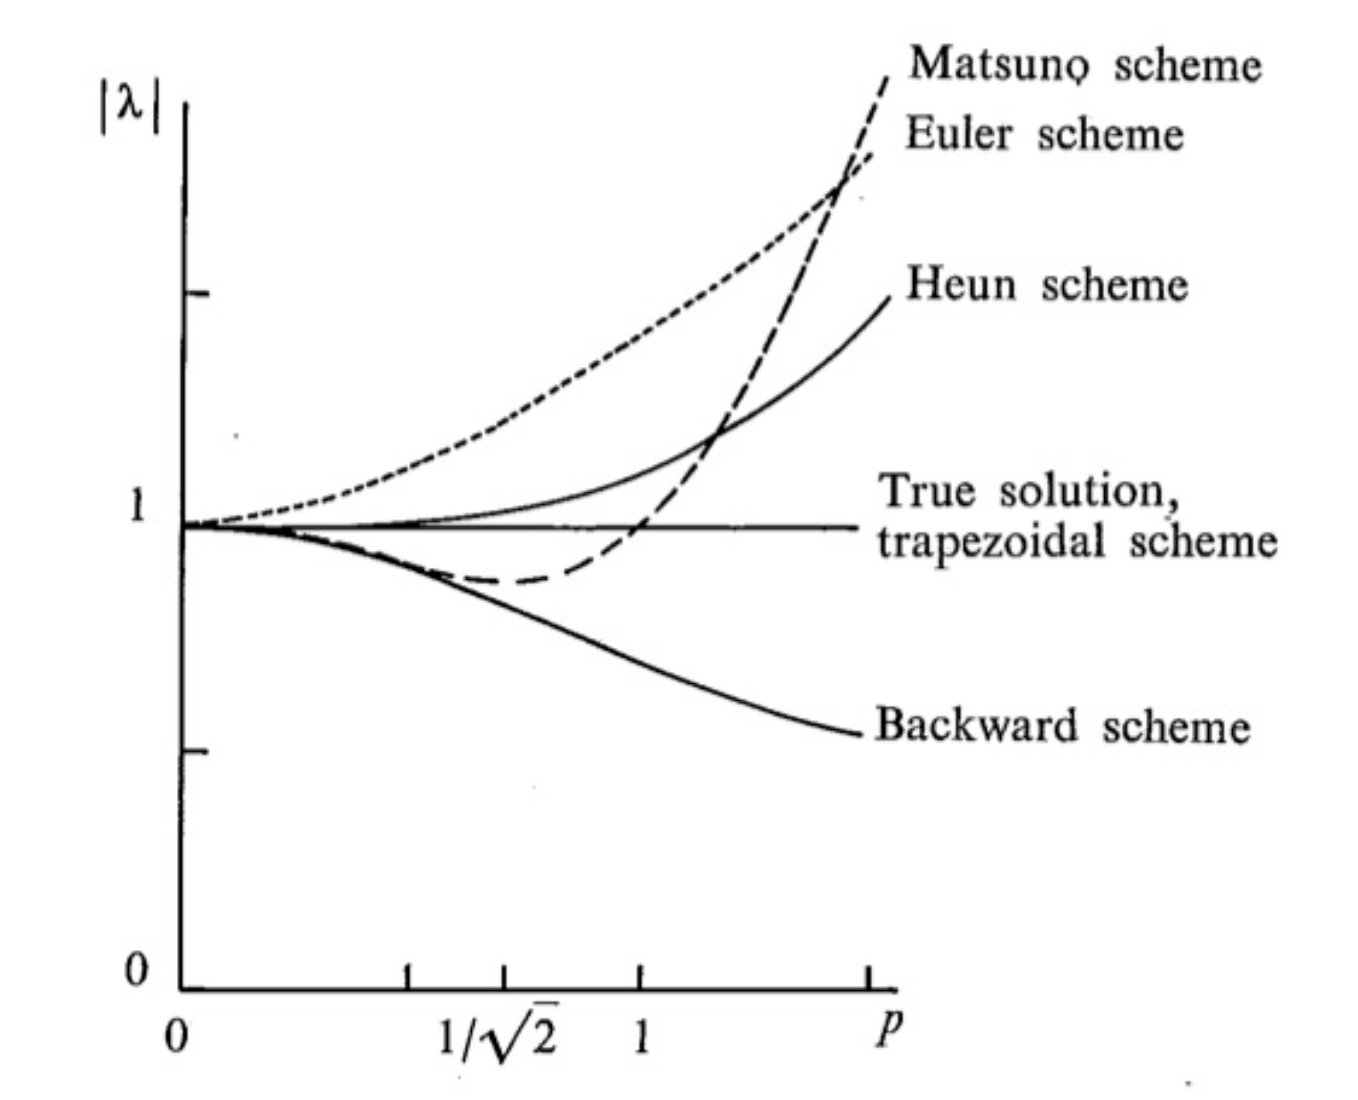
\includegraphics[width=0.50\linewidth]{uploads/Screenshot 2024-11-12 101958.png}
	\caption{The amplification factor as a function of $p=\omega\Delta t$, for the five two level schemes and for the true solution}
	\label{fig:3.2.1}
\end{figure}
Figure \ref{fig:3.2.1} summarizes the results obtained for the five schemes considered so far. For all of these schemes the amplification factors were found to be even functions of $p$, so the amplification factor curves are shown only for $p\geq 1$.
\paragraph{Leap-Frog scheme (Three level schemes)}
The more accurate leap-frog scheme is more delicate.
\begin{equation}\label{3.2.33}
	U^{(n+1)}=(U^{(n-1)}+2i\omega\Delta tU^{(n)}
\end{equation}
A problem with all three or more level schemes including this is that they require more than one initial condition to start the computation. From a physical standpoint a single initial condition $U^{(0)}$ should have been sufficient. However, in addition to the physical initial condition, three level schemes require a computational initial condition $U^{(1)}$. This value cannot be calculated by a three level scheme, and, therefore, it will usually have to be obtained using one of the two level schemes. According to \ref{3.2.3} we also have
\begin{equation}\label{3.2.34}
	U^{(n)}=\lambda U^{(n-1)}\,\,\, U^{(n+1)}=\lambda^2U^{(n-1)}
\end{equation}
substitued in \ref{3.2.33} we have
$$\lambda^2-2ip\lambda-1=0$$ that has solutions:
\begin{align*}
	\lambda_1=\sqrt{1+p^2}+ip \\
	\lambda_2=-\sqrt{1-p^2}+ip
\end{align*}
Thus, there are two solutions of the form $U^{(n+1)}=\lambda U^{(n)}$. This necessarily follows from the fact that we are considering a three level scheme; substitution of \ref{3.2.34} into the difference equation given by these schemes will always give a second degree equation for $\lambda$. In general, an m level scheme will give $m — 1$ solutions of the form $U^{(n+1)}=\lambda U^{(n)}$. A solution of this type corresponding to a single value of $\lambda$ is called a mode.

Consider now the two values that have been obtained for $\lambda$. If a solution of the form $U^{(n+1)}=\lambda U^{(n)}$ is to represent an approximation to the true solution, then we must have $\lambda\rightarrow 1$ as $\Delta t\rightarrow0$. For the values $\lambda_1, \lambda_2$, as $p=\omega\Delta t\rightarrow0$ we do have $\lambda_1\rightarrow1$, however at the same time $\lambda_2\rightarrow-1$. Solutions like that associated with $\lambda_1$ are usually called \textit{physical modes} because we are always solving equations describing physical processes. Solutions like that associated with $\lambda_2$ are not approximations to the true solution, and are called \textit{computational modes}.
\begin{itemize}
	\item Case $|p|<1$: then $|\lambda|=1$ stable
	\item Case $|p|=1$: then $|\lambda|=1$ equal
	\item Case $|p|>1$: then $|\lambda|=|p\pm\sqrt{p^2-1}|$ unstable
\end{itemize}
\subsubsection{Stability for dissipation equation}
For the dissipation equation
\begin{equation}\label{3.3.6}
	\frac{dU}{dt}=-kU \text{,} \,\, U=U(t)\text{,} \,\, k>0
\end{equation}
Again it is easy to justify our interest in this equation. For example, if we define $U=u+iv$, it describes the effect of friction proportional to the velocity vector, as is often assumed for motions near the ground. As another example, note that when seeking a solution of the heat transfer, or Fick’s diffusion equation in the form od a single harmonic component.
The general solution of \ref{3.3.6} is
\begin{equation}
	U(t)=U(0)e^{-kt}
\end{equation}
Thus, both the real and the imaginary part decrease exponentially with time.
The properties of schemes applied to \ref{3.3.6} will again be analyzed using the von Neumann method. As in the previous section, we consider first the non-iterative two level scheme \ref{3.2.6}. Applied to the diffusion equation, it gives:
\begin{equation}\label{3.3.8}
	U^{(n+1)}=U^{(n)}-k\Delta t\left(\alpha U^{(n)}+\beta U^{(n+1)}\right)
\end{equation}
writing $K=k\Delta t$ we have
\begin{equation}\label{3.3.10}
	U^{(n+1)}=\frac{1-\alpha K}{1+\beta K}U^{(n)}
\end{equation}
and
\begin{equation}
	\lambda=\frac{1-\alpha K}{1+\beta K}
\end{equation}
For the two level schemes we have:
\begin{itemize}
	\item Euler ($\alpha=1, \beta=0$): $\lambda=|1-K|\rightarrow0<K\leq2$ stable
	\item Backward ($\alpha=0, \beta=1$): $\lambda=\frac{1}{1+K}\rightarrow K>0$ stable
	\item Trapezoidal ($\alpha=1/2, \beta=1/2$): $\lambda=\frac{1-1/2K}{1+1/2K}\rightarrow K>0$ stable
\end{itemize}
while for the leap-frog scheme:
$$\lambda^2+2K\lambda-1=0$$
giving the solutions
\begin{align}
	\lambda_1=-K+\sqrt{1+K^2} \\
	\lambda_2=-K-\sqrt{1+K^2}\notag
\end{align}
As $k\rightarrow0$, $\lambda_1\rightarrow1$, while $\lambda_2\rightarrow-1$ thus, the solution associated with $\lambda_1$ again represents the physical mode, and that associated with $\lambda_2$ the computational mode. For  $K>0$, that is for the normal case of a forward integration in time,  this  result  always  in  a  computational  mode $\lambda_2$  that  is always  unstable. It changes sign from time step to time step, and its magnitude increases. As before, we cannot hope to eliminate the computational mode completely. Because  we  can’t  eliminate  completely  the computational   mode   the   leapfrog   cannot   be   used   for   the dissipation equation.
The  same  analysis  applied  to  the  friction  equation  will  give  a different  result.  The  Euler  scheme  is  stable  and  the  leapfrog scheme is instead is always unstable.
\subsection{A combination of schemes}
A natural question to ask at this point is what can we do if, for example, the equation contains both the oscillation and the dissipation term, that is
\begin{equation}\label{3.4.1}
	\frac{dU}{dt}=i\omega U-kU
\end{equation}
Here we might like to use the leapfrog scheme because of the oscillation term $i\omega U$, but we know that it cannot be used for the dissipative term $-kU$. In this and similar situations we can use different schemes for the different terms; for example, we might use the leapfrog scheme for the oscillation term and the forward scheme for the dissipative term. We then obtain:
\begin{equation}
	U^{(n+1)}=U^{(n-1)}+2\Delta t\left(i\omega U^{(n)}-kU^{(n-1)}\right)
\end{equation}
\section{The Advection Equation}
We now consider differential equations with one dependent and two or three independent variables, that is, partial differential equations. More specifically, we shall consider various simplified forms of the advection equation, describing advection of a dependent variable. This is considered in practice to be the most important part of the atmospheric governing equations.

We have already discussed the one-dimensional linear advection equation to some extent in the introductory chapter. We shall organize the analysis here so as first to continue considering problems associated with the simplest one-dimensional linear form of the advection equation, and then to proceed to problems introduced by more complex forms of the advection equation.
Consider the equation
\begin{equation}\label{4.1.1}
	\frac{\partial u}{\partial t}+c\frac{\partial u}{\partial x}=0
\end{equation}
here $u=u(x,f)$ is a function of two independent variables: the independent variable $x$ will represent a space variable, and, thus, \ref{4.1.1} will be called the one-dimensional linear advection equation. As seen earlier, its general solution is
$$u=f(x-ct)$$ where $f$ is an arbitrary function.
One of the finite difference schemes for \ref{4.1.1} is the forward and upstream scheme. If the space derivative (i.e. discretizing only "$x$") is approximated by a centered finite difference quotient using values at the two nearest points, we obtain for the time derivative:
\begin{equation}\label{4.1.3}
	\frac{\partial u_j}{\partial t}=-c\frac{u_{j+1}-u_{j-1}}{2\Delta x}
\end{equation}
The subscript here, as before, denotes the distance from the origin in space increments; that is, $x=j\Delta x$. A number of schemes for the numerical solution of \ref{4.1.1} can now be constructed because we can approximate the time derivative in \ref{4.1.3} by one of the methods studied in the preceding chapter. For example, when the time derivative is approximated using the leapfrog scheme, we obtain
\begin{equation}\label{4.1.4}
	\frac{u^{n+1}_j-u^{n-1}_j}{2\Delta t}=-c\frac{u_{j+1}^n-u_{j-1}^n}{2\Delta x}
\end{equation}
as one of many possible consistent schemes for the numerical solution of \ref{4.1.1}.

A possible solution of \ref{4.1.1} will be of the form
\begin{equation}\label{4.1.5}
	u_j=\text{Re}\left[U(t)e^{ikj\Delta x}\right]
\end{equation}
going back to the oscillation equation:
\begin{equation}\label{4.1.6}
	\frac{dU}{dt}=i\left(-\frac{c}{\Delta t}\sin k\Delta x\right)U
\end{equation}
denoting
$$p=-c\frac{\Delta t}{\Delta x}\sin k\Delta x$$
Now, if we approximate \ref{4.1.6} using one of the time differencing schemes, the same finite difference equation is obtained as when we apply that scheme to \ref{4.1.3} and then substitute the wave solution \ref{4.1.5}. Hence, properties of finite difference schemes derived from \ref{4.1.3} can be inferred from the results of Section Time differencing schemes, where the frequency to is given by $p=\omega\Delta t$.
As an example, if \ref{4.1.6} is approximated using the leap-frog scheme, we obtain:
\begin{equation}\label{4.1.8}
	U^{(n+1)}=U^{(n-1)}+2\left(-c\frac{\Delta t}{\Delta x}\sin k\Delta x\right)U^{(n)}
\end{equation}
with
\begin{equation}\label{4.1.9}
	p=-c\frac{\Delta t}{\Delta x}\sin k\Delta x
\end{equation}
We obtain the same finite difference equation \ref{4.1.8} by first applying the leapfrog scheme to \ref{4.1.3} giving \ref{4.1.4} and then substituting \ref{4.1.5} into \ref{4.1.4}. Thus, properties of \ref{4.1.4} can be inferred from the known properties of the leapfrog scheme applied to the oscillation equation.

Let us look at some of conclusions obtained in this way. For stability of the leapfrog scheme it was required that the condition $|p|\leq 1$ occuring. Thus, we have to satisfy
\begin{equation}
	\left|c\frac{\Delta t}{\Delta x}\sin k\Delta x\right|\leq 1
\end{equation}
for any admissible $k$. Since $|\sin k\Delta x|$ does reach the maximum value of unity in the admissible range of $k$, we obtain the stability condition
\begin{equation}\label{4.1.10}
	|c|\frac{\Delta t}{\Delta x}\leq 1
\end{equation}
This critetion (already mentioned) shows that stability cannot simply be anchieved by reduction of the time and space increments. Rather, it is necessary to reduce the ratio of these increments $\frac{\Delta x}{\Delta t}$ to obtain stability. This condition was first found by Courant, Friedrichs and Lewy (1928) and therefore, is usually referred to as the Courant-Friedrichs-Lewy, or CFL. stability criterion.

It is instructive to note that the maximum value of $|p|$, that is, the minimum stability, is associated with the wave with $k\Delta x=\frac{\pi}{2}$. This is the component with wave length $4\Delta x$, twice the shortest resolvable wave length $2\Delta x$.


Let us use now another scheme to approximate the time derivative in \ref{4.1.3}: the Matsuno scheme. First the approximate values $u_j^{(n+1)*}$ using the forward scheme, that is,
\begin{equation}\label{4.1.16}
	\frac{u_j^{(n+1)*}-u_j^n}{\Delta t}+c\frac{u^n_{j+1}-u^n_{j-1}}{2\Delta x}=0
\end{equation}
then, these approximate values are used in the backward scheme, that is,
\begin{equation}\label{4.1.17}
	\frac{u_j^{(n+1)}-u_j^n}{\Delta t}+c\frac{u_{j+1}^{(n+1)*}-u_{j-1}^{(n+1)*}}{2\Delta x}=0
\end{equation}
eliminating the intermediate step, i.e. the approximate values $u^{(n+1)*}$ , from this equation, by substituting values given by \ref{4.1.16}, with the subscript $j$ replaced by $j+1$ and then by $j-1$.
\begin{align*}
	\frac{u_{j+1}^{(n+1)*}-u_{j+1}^n}{\Delta t}+c\frac{u_{j+2}^{n}-u_{j}^{n}}{2\Delta x}=0 \\
	\frac{u_{j-1}^{(n+1)*}-u_{j-1}^n}{\Delta t}+c\frac{u_j^{n}-u_{j-2}^{n}}{2\Delta x}=0
\end{align*}
CFL criterion.
In this way we obtain:
\begin{equation}\label{4.1.18}
	\frac{u_j^{(n+1)}-u_j^n}{\Delta t}=-c\frac{u_{j+1}^{n}-u_{j-1}^{n}}{2\Delta x}+c^2\frac{u^n_{j+1}-2u^n_j+u^n_{j-2}}{2\Delta x^2}
\end{equation}
Without the last term, this represents the finite difference equation obtained when the forward scheme is used for the time derivative in \ref{4.1.3}. The third term approaches zero as $\Delta x,\Delta t\rightarrow 0$, and \ref{4.1.18} is therefore also a consistent scheme for the advection equation. On the other hand, for a fixed $\Delta t$ this term approaches $c^2\Delta t\left(\frac{\partial^2u}{\partial x^2}\right)$ as $\Delta x\rightarrow0$. It is therefore of the same form as a finite difference approximation to a Fick’s diffusion term, and it has a damping effect. This damping effect, however, is dependent on the wave length. As the third term is calculated over an interval of $4\Delta x$, the maximum damping occurs for a wave with wave length of $4\Delta x$. There is no damping of the shortest resolvable wave with wave length $2\Delta x$. Even if a damping effect were desirable when solving the advection equation, we would not want this particular dependence on wave length. Thus, the Matsuno scheme does not appear suitable for solving the advection equation.

It is convenient to include here one more example of the use of the energy method for testing stability. In addition to being applicable also to nonlinear equations, it can be used to study the effect of boundary conditions on stability. We will use the energy method here to test the stability of a group of schemes that can be used for solving \ref{4.1.3}.
The last term can be decomposed as
\begin{equation}
	\frac{u_{j+1}^n-2U_j^n+u_{j-2}^n}{2\Delta x^2}=\left(\frac{u^n_{j+2}-u^n_j}{2\Delta x}\right)-\left(\frac{u_j^n-u^n_{j-2}}{2\Delta x}\right)\frac{1}{2\Delta x}\approx \frac{\partial^2u}{\partial x^2}
\end{equation}
\begin{figure}[h]
	\centering
	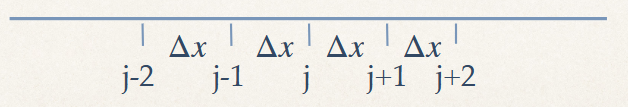
\includegraphics[width=0.5\linewidth]{uploads/Screenshot 2024-11-12 151817.png}
	\caption{steps}
	\label{fig:step}
\end{figure}
The scheme is adding a dissipative term.
\subsubsection{Non linear advection}
Consider now the non-linear advection equation
\begin{equation}\label{4.6.5}
	\frac{\partial u}{\partial t}=-u\frac{\partial u}{\partial x}
\end{equation}
consider the effect of the non linear term on a single wave $u=\sin kx$, a function $u(x)$ which can be represented by values at grid points. When performed on finite differences it cannot resolve wave length shorter than $2\Delta x$, or wave numbers greater than $k_{max}=\pi/\Delta x$,  $k<k_{max}$.
For the wave the non-linear term will look like:
\begin{equation}
	u\frac{\partial u}{\partial x}=k\sin kx\cos kx=\frac{1}{2}k\sin 2kx
\end{equation}
If $k$ is in the range $\frac{1}{2}k_{max}<k\leq k_{max}$ the result of the multiplication will be beyond the capability of the grid to represent. It cannot, therefore, be properly reproduced in a finite difference calculation.
To gain some insight into what happens in such a situation, consider a wave for which $k>K_{max}$. For example, let $L_t=\frac{4\Delta x}{3}$. A wave of that wave length is shown by the full line in 4.6.2. Knowing only the values at grid points we will not be able to distinguish this wave from the one shown by the dashed line. Thus, with the convention adopted earlier which assumes that the longest waves are present, we will make an error. This is called \textit{aliasing error}.
\begin{figure}[h]
	\centering
	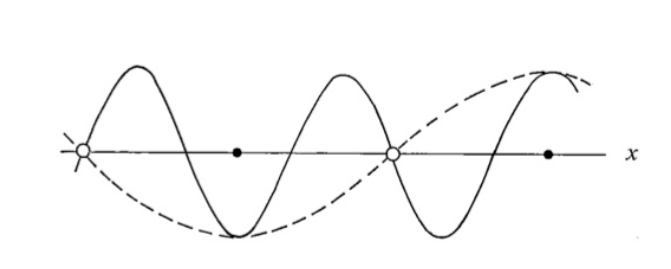
\includegraphics[width=0.5\linewidth]{uploads/Screenshot 2024-11-12 161236.png}
	\caption{A wave of wave length $\frac{4\Delta x}{3}$, misrepresented by the finite difference grid as a wave of wave length $4\Delta x$.}
	\label{fig:4.6.2}
\end{figure}
The waves with wave number $k_u>k_{max}$ will be interpreted as longer waves according to $k^*=2k_{max}-k_u$.
In a real numerical solution, higher wave numbers will be continuously be created by the non linear interactions and so the amplitude of wave numbers close to $k_{max}$ will continue to increase.\\
[0.4cm]

Now consider the consequences of aliasing errors in a numerical integration. An atmospheric variable, as a function of space co-ordinates, can be thought of as consisting of a series of harmonic components. It is useful to consider the “energy” of these components, that is, their contribution to the mean square value of the variable considered as a function of wave number.

This is the \textit{spectrum} of the “energy”. For example, if the variables are velocity components, this function is the kinetic \textit{energy spectrum}. This spectrum describes the relative importance of features of different scales in the field of the variable. Now, experience shows that the spectrum of atmospheric variables does not change much with time. On synoptic maps we do not have situations where small scale features are dominant on one day, and absent on the next. Accordingly, spectra of atmospheric variables also do not change much in their general shape. The energy of a particular component can, of course, change, but the characteristic shape of the spectrum as a whole is fairly constant. For example, a zonal spectrum of the eastward velocity component in middle latitudes typically has a maximum for wave numbers 4 to 7, that is, 4 to 7 wave lengths along a latitude circle, with the energy tapering off rather rapidly as the wave number increases beyond about 10. Thus, there is very little energy in wave numbers of the order of the maximum wave numbers that can be resolved by finite difference grids used in atmospheric models.

In a finite difference integration, in addition to these relatively small physical changes, the shape of a spectrum is subject to changes due to aliasing errors. If we have a spectrum of the shape just described, and consider the representation of various combinations $k_1+k_2$ that are greater than $k_{max}$, we see that most of the energy of such combinations will belong to components with wave numbers not much greater than $k_{max}$ . Thus, due to aliasing errors a spurious energy inflow is expected at wave numbers that are not much less than $k_{max}$, and, in time, the energy of these components can be expected to grow beyond physically acceptable limits. Experience shows that, if no precautionary measures are taken, this can indeed happen, and even cause a catastrophic end to the integration. The phenomenon is due to the nonlinear terms of the equations, and, therefore, is called the \textit{nonlinear instability}. Nonlinear instability was first encountered by Norman Phillips (1956) in his famous work that laid the foundation for the numerical modeling of the atmospheric general circulation. Starting from an atmosphere at rest, he integrated the vorticity equation for a simulated time of the order of 30 days. The calculation then came to an end due to an explosive increase in the total energy of the system, associated with an appearance of elongated shapes in the vorticity field. Phillips initially believed that the breakdown was due to excessive truncation errors, and he later repeated the experiment using space and time steps both reduced to about half of their previous values. This must have greatly reduced the truncation errors, but the catastrophic increase in total energy still happened at about the same time.

In a later paper Phillips (1959) gave the interpretation of nonlinear instability similar to what has been presented here, but for the nondivergentvorticity equation. For a test of this explanation Phillips again repeated his experiment, but after every two hours of simulated time he performed a harmonic analysis of the vorticity fields, and eliminated all components with $k>\frac{1}{2}k_{max}$. If there are no components with $k>\frac{1}{2}k_{max}$ the advection term cannot produce waves with $k>k_{max}$. We expect that it will be some time before the amplitudes of the eliminated waves are built up again to an appreciable extent. This filtering procedure eliminated the appearance of the spurious increase in energy, thereby confirming this explanation of the instability.
\section{Energy and numerical methods}\label{sec:en and numerical methods}
\begin{center}
	\textit{References for the following section can be found in the book at chapter 4.2: Finite differencing in two dimensions}
\end{center}

Some issues with nonlinear instability:
\begin{itemize}
	\item The nonlinear instability shows the issues with controlling errors that make the amplitude grow indefinitely
	\item On the other end, this issues shows that there are conservation property of the basic equations that must be reflected in the numerical scheme.
	\item This remark led to the development or the requirement that numerical scheme must be devised that have the same conservation properties of the original equation
	\item To illustrate this point we will use the simplified homogeneous flow system that we have introduced previously.
\end{itemize}
The selection of appropriate spatial finite difference formulations to use in the horizontal and vertical directions varies widely depending on which properties are being modeled or are considered important. Most climate models are not intended primarily for predicting the exact location of daily weather events with great accuracy but are directed more toward the simulation of the long-term mean and variance states of the climate system. Since the models frequently run for long periods of time, the numerical schemes used should approximately maintain many of the integral constraints that are in the original differential equations, such as conservation of mass, energy and momentum. Many climate models have employed horizontal finite difference methods that maintain these features.

Consider an incompressible fluid with a variable height, and assume that the horizontal velocity components, $u$ and $v$ are independent of height, and that the vertical velocity $w$ equals 0 at the bottom of the fluid. The set of momentum equations for a homogeneous flow are the following:
$$h=0$$
\begin{align}\label{eq.momentum}
	\frac{\partial u}{\partial t}=-u\frac{\partial u}{\partial x}-v\frac{\partial u}{\partial y}+fv-g\frac{\partial\eta}{\partial x}       \\
	\frac{\partial v}{\partial t}=-u\frac{\partial v}{\partial x}-v\frac{\partial v}{\partial y}-fu-g\frac{\partial\eta}{\partial y}\notag \\
	\frac{\partial \eta}{\partial t}=-\frac{\partial}{\partial x}u(\eta+H_0)-\frac{\partial }{\partial y}v(\eta+H_0)\notag
\end{align}
Considering the total height $H=H_0+\eta$ and multiplying the first two equations by $H$ we obtain:
\begin{align*}
	H \frac{\partial u}{\partial t}=-uH\frac{\partial u}{\partial x}-vH\frac{\partial u}{\partial y}+fHv-gH\frac{\partial\eta}{\partial x} \,\,\, \text{(1)} \\
	H\frac{\partial v}{\partial t}=-uH\frac{\partial v}{\partial x}-vH\frac{\partial v}{\partial y}-fHu-gH\frac{\partial\eta}{\partial y}\,\,\, \text{(2)}   \\
	\frac{\partial H}{\partial t}=-\frac{\partial}{\partial x}uH-\frac{\partial }{\partial y}vH \,\,\, \text{(3)}
\end{align*}
Using the relations:
\begin{equation}
	H\frac{\partial u}{\partial t}=\frac{\partial}{\partial t}(uH)-u\frac{\partial H}{\partial t}=-\frac{\partial}{\partial x}(uuH)+u\frac{\partial}{\partial x}(uH)-\frac{\partial}{\partial x}(uvH)+u\frac{\partial}{\partial x}(vH)
\end{equation}
We can rewrite the equations of motion as:
\begin{align}
	\frac{\partial uH}{\partial t}=-\frac{\partial uuH}{\partial x}-\frac{\partial uvH}{\partial y}+fHv-g\frac{\partial\eta}{\partial x}        \\
	\frac{\partial vH}{\partial t}=-\frac{\partial uvH}{\partial x}-\frac{\partial vvH}{\partial y}-fHu-gH\frac{\partial\eta}{\partial y}\notag \\
	\frac{\partial H}{\partial t}=-\frac{\partial}{\partial x}uH-\frac{\partial }{\partial y}vH\notag
\end{align}
In this form the mass equation makes mass conservation immediately visible, let us now consider energy.
Kinetic energy is defined as:
$$KE=\frac{1}{2}H(u^2+v^2)$$
and the potential energy:
$$PE=\frac{1}{2}gH^2$$
now, by multiplying eq.(1) by $Hu$ and (3) by $u^2/2$ and adding, then eq. (2) by $Hv$ and (3) by $v^2/2$ and adding, using the product derivative rule as before, we can get:
\begin{align}
	\frac{\partial}{\partial t}\left(H\frac{1}{2}u^2\right)+\frac{\partial}{\partial x}\left(Hu\frac{1}{2}u^2\right)+\frac{\partial}{\partial y}\left(Hv\frac{1}{2}u^2\right)-fHvu+gHu\frac{\partial H}{\partial x} \\
	\frac{\partial}{\partial t}\left(H\frac{1}{2}v^2\right)+\frac{\partial}{\partial x}\left(Hu\frac{1}{2}v^2\right)+\frac{\partial}{\partial y}\left(Hv\frac{1}{2}v^2\right)-fHvu+gHv\frac{\partial H}{\partial x} \\
\end{align}
multiplying the continuity equation (3) by $gH$ and rearranging we get:
\begin{equation}
	\frac{\partial}{\partial t}\left(g\frac{1}{2}H^2\right)+\frac{\partial}{\partial x}\left(gH^2u\right)+\frac{\partial}{\partial y}\left(gH^2v\right)-gH\left[u\frac{\partial H}{\partial x}+v\frac{\partial H}{\partial y}\right]=0\\
\end{equation}
The total energy is defined as:
$$TE=KE+PE=\frac{1}{2}H(u^2+v^2)+\frac{1}{2}gH^2$$
hence,
\begin{equation}
	\frac{\partial}{\partial t}TE=\frac{\partial }{\partial x}\left(\frac{Hu}{2}(u^2+v^2)+gH^2\right)+\frac{\partial}{\partial y}\left(\frac{Hv}{2}(u^2+v^2)+gH^2\right)
\end{equation}
Integrating over the domain assuming periodic boundary conditions, we get the result for the time variation of the total energy. The integration of the boundary terms is zero and so we get the final result showing the conservation of the total energy.
\subsection{Conservation in numerical schemes}
Let's go back to the simple problem
\begin{equation}
	\frac{\partial u}{\partial t}=-u\frac{\partial u}{\partial x}=-\frac{\partial}{\partial x}\left(\frac{u^2}{2}\right)
\end{equation}
In numerical form (any schemes would do) for a centered difference scheme:
\begin{equation}
	\frac{\partial u}{\partial t}\approx -\frac{u^2_{j+1}-u^2_{j-1}}{4\Delta x}
\end{equation}
The energy will be the sum over the grid point values.
\begin{equation}
	\int\frac{\partial}{\partial t}u^2=\int u\frac{\partial}{\partial t}u\approx\displaystyle\sum_{j=1}^{N-1}\frac{u^2_{j+1}-u^2_{j-1}}{4\Delta x}u_j
\end{equation}
If we expand the sum we notice that terms do not compensate each other so the scheme does not conserve energy. The problem arise from the terms that are mixed in a way that does not compensate. However, in the original equation there are compensations, so maybe we can find ways of writing the equations in a equivalent way.
$$
	\frac{\partial u}{\partial t}=-\frac{1}{3}\left[u\frac{\partial u}{\partial x}+\frac{\partial}{\partial x}u^2\right]
$$
using the same centered scheme:
$$\frac{\partial u}{\partial t}\approx -\frac{1}{3}\left[u_j\frac{u_{j+1}-u_{j-1}}{2\Delta x}+\frac{u^2_{j+1}-u^2_{j-1}}{2\Delta x}\right]
$$
will result in a scheme that conserves energy. So, by using alternative but equivalent formulations schemes with desirable conservation properties can be found.

We have seen how find a different thing can be used to solve one-dimensional problems. But the real world is of course three dimensional and we have to understand how to deal with that in order to attack realistic cases. Therefore it is important that we understand how we can apply these methods to more dimensions. To address the problem in more dimensions, let's first introduce a key feature of numerical modeling.
\subsection{The Arakawa Jacobian}
The Arakawa Jacobian is central to numerical modeling in geophysical fluid dynamics, particularly for ensuring the conservation and stability of numerical simulations of vorticity and enstrophy (a measure of the vorticity squared). This concept is foundational in finite-difference schemes used to model fluid flows, such as weather patterns or ocean currents.


A conceptually elegant approach for dealing with the nonlinear instability problem has been suggested and developed by Arakawa (1966, 1972). His idea is that it is better, if possible, to use schemes for the advection terms that are not only free of the nonlinear computational instability but also free of the spurious inflow of energy to these short waves, instead of artificially suppressing their amplitudes. The amplitudes of the shortest waves in atmospheric models are small initially, and they will remain small if a false generation of these short waves is avoided. Arakawa has shown that it is possible to construct such schemes, and that they are obtained when care is taken to conserve in the finite difference form some integral properties of the original differential equations.

When the Arakawa conservation schemes are used there is no need for an artificial dissipation in the advection process. This enables the statistical properties of the schemes to be maintained under advection, a feature especially useful in general circulation studies.

Here are the key points and essential concepts regarding the Arakawa Jacobian and its application in two finite-difference schemes. The Arakawa Jacobian is a numerical method used to approximate the Jacobian term in the vorticity equation of fluid dynamics, which is the nonlinear term representing the interaction of velocity fields. This term is crucial in the conservation of key quantities like energy and enstrophy, both of which need to be carefully handled to avoid numerical artifacts and to accurately represent physical processes in models.



A major advantage of the Arakawa scheme is its ability to eliminate nonlinear instability, which arises due to the accumulation of energy at small scales caused by aliasing. By carefully constructing the Jacobian, the scheme conserves both energy and enstrophy, preventing the unphysical growth of energy in smaller scales.

There are many ways of constructing finite difference approximations to the Jacobian. We can use any of the three equivalent analytic expressions. We shall consider only approximations of the second order of accuracy. With the simplest centered space differencing, we require values of $p$, $q$ from a box of nine adjacent grid points to evaluate the Jacobian.
\begin{figure}[h]
	\centering
	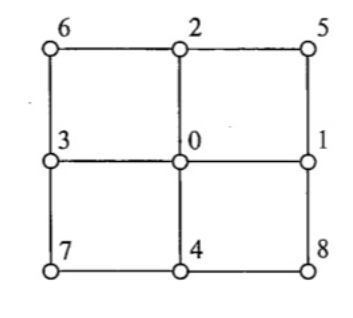
\includegraphics[width=0.25\linewidth]{uploads/Screenshot 2024-11-13 174915.png}
	\caption{Stencil used to define approximations to Jacobian}
	\label{fig:4.7.2}
\end{figure}

The construction of the Arakawa Jacobian involves combining multiple second-order approximations, denoted as $J^{++},J^{x+},J^{+x}$, with specific weights chosen to conserve energy, enstrophy, and vorticity.
The superscripts $+$ and $x$ denote the positions of the points from which values of $p$ and $q$, respectively, are used to form the approximation. Each of the approximations $J^{++}$, $J^{+x}$ and $J^{x+}$ is consistent and of the second order of accuracy. A more general approximation can now be formed as a linear combination of these three, that is
$$J(p,q)=\alpha J^{++}+\beta J^{x+}+\gamma J^{+x}$$ with $\alpha+\beta+\gamma=1$.
To illustrate that let's use the vorticity equation in the non-divergent form:
\begin{equation}\label{nondivvor}
	\frac{\partial}{\partial t}\nabla^2\psi+J(\psi, \nabla^2\psi+f_0+\beta y)=0
\end{equation}
The nonlinear instability was generated by the nonlinear advection terms that are represented here by the Jacobian operator $J(\psi, \nabla^2\psi)$. So the term that we have to treat carefully is the Jacobian. The Arakawa Jacobian, that has been used by essentially every climate model using finite differences, is
$$J_A=\frac{1}{3}\left(J^{++}+J^{x+}+ J^{+x}\right)$$
By eliminating the need for artificial dissipation, the scheme preserves the statistical properties of advection, making it particularly valuable for general circulation and climate studies. The Arakawa scheme also controls the computational energy cascade by conserving the average wave number in the advection terms of the nondivergent flow, addressing nonlinear instability more effectively than simpler energy-conserving approximations.

Interestingly, the Arakawa Jacobian has been demonstrated to be a special case of the finite element method, where a variational formulation minimizes errors through interpolation. However, while the scheme ensures conservation of energy and enstrophy, these properties alone do not guarantee the accuracy of the solution. Thus, the Arakawa Jacobian remains a powerful tool for controlling numerical instability, even though solution accuracy must be verified through additional means.



Thus, it is not only a conservation of energy, as has sometimes incorrectly been implied. For example, an approximation can easily be constructed for the non­linear term of the one-dimensional advection equation \ref{4.6.5} which would conserve the kinetic energy. Using such an approximation, however, would not prevent nonlinears instability in the way that the Arakawa scheme does. The Arakawa procedure does not have a one-dimensional analogue, as the non-divergent vorticity equation \ref{nondivvor} is not nonlinear when applied to a one-dimensional problem.


\subsection{Gravity waves}
In this chapter we consider the equations describing the horizontal propagation of gravity and gravity-inertia waves. Mathematically, this means that we will be dealing with a system of two or three partial differential equations of the first order. Thus, we will now have two or three dependent variables. The system of equations will always be equivalent to a single differential equation of a higher order. This equation can be obtained from the system by elimination of dependent variables.

We first put this problem in perspective. Arakawa, (Arakawa, 1970), has stated that there are two main problems in finite difference integrations of the atmospheric governing equations. One is a proper simulation of the geostrophic adjustment process. Through this process the atmosphere establishes a characteristic quasi-non divergent state, mostly as a result of the dispersion of the gravity-inertia waves. The associated computational considerations will be discussed in this chapter. The second problem is the prediction or simulation of the large-scale quasi-non divergent flow after it has been established. Here the horizontal advection is the dominating mechanism.

Extensive study of the problems in integrations of the gravity-inertia wave equations began in atmospheric modeling much later than studies of the advection problem. After Richardson’s (1922) first unsuccessful numerical integration of the complete primitive equations, the successful result of Charney, Fjortoft and von Neumann (1950) was largely due to the exclusion of gravity-inertia waves from their equations by using the geostrophic approximation in the vorticity equation. The governing equations with the gravity-inertia waves excluded, are customarily called the filtered equations. They bypass the geostrophic adjustment problem. The filtered equations were used almost exclusively in the first decade of numerical forecasting research.

Efforts to improve the performance of numerical models led to a desire to include the non-geostrophic effects. This is very difficult to do within the modified system of equations. Thus, starting with the first successful experiments by Hinkelmann (1959), modelers came back to using the primitive equations. Except for special purposes, the primitive equations are used almost
exclusively in atmospheric models today. They are generally considered superior for both research and operational applications (e.g. Sawyer, 1972). The speed of propagation of the gravity and gravity-inertia waves, and their sensitivity to various numerical errors mean that their treatment requires especially careful consideration.

The more general case of one dimension the gravity waves:
\begin{align*}
	\frac{\partial u}{\partial t}=-g\frac{\partial H}{\partial x} \\
	\frac{\partial H}{\partial t}=-H_0\frac{\partial u}{\partial x}
\end{align*}
will generate the differencing:
\begin{align}\label{5.1.6}
	\frac{\partial u_j}{\partial t}=-g\frac{H_{j+1}-H_{j-1}}{2\Delta x} \\
	\frac{\partial H_j}{\partial t}=-H_0\frac{u_{j+1}-u_{j-1}}{2\Delta x}
\end{align}
with \begin{equation}\label{5.1.10}
	c^*=\pm\sqrt{gH_0}\frac{\sin k\Delta x}{k\Delta x}
\end{equation}
This phase speed is a function of wave number, and, thus, we see that the space differencing again results in computational dispersion. The formula \ref{5.1.10} is the same as the one obtained in the preceding chapter when considering the advection equation. Therefore, both the phase speed and the group velocity depend on the wave number. The phase speed decreases as the wave length decreases, and the wave with wave length $2\Delta x$ is stationary.

There is, however, an important difference between this problem and the advection problem because we now have two dependent variables. We have assumed that they are both carried at every grid point.\begin{figure}[h]
	\centering
	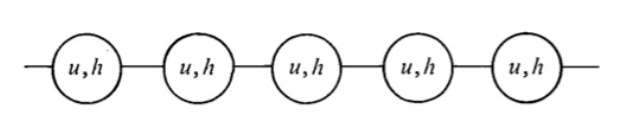
\includegraphics[width=0.5\linewidth]{uploads/Screenshot 2024-11-13 180623.png}
	\caption{A grid with two dependent variables that are both carried at every grid points.}
	\label{fig:5.1.3}
\end{figure}
As far as the system \ref{5.1.6} is concerned, however, the underlined variables in the figure depend only on other underlined variables. The same statement holds for the variables that are not underlined. Thus, the grid in the figure contains two elementary “sub-grids”, with the solution on one of these sub-grids being completely decoupled from the other. Thus, it would be better to calculate only one of these solutions, that is, to use a grid as shown below in \ref{fig:5.1.4} Such a grid, with variables carried at alternate points in space, is called a staggered grid.
\begin{figure}[h]
	\centering
	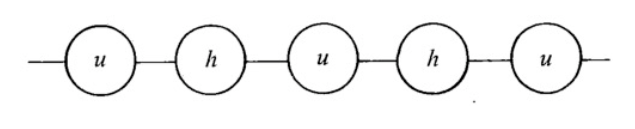
\includegraphics[width=0.5\linewidth]{uploads/Screenshot 2024-11-13 180824.png}
	\caption{A grid with two dependent variables that are carried at alternate grid points.}
	\label{fig:5.1.4}
\end{figure}
The computation time needed to solve \ref{5.1.6} on the grid is reduced by a factor of two, and the truncation error is the same. Furthermore, the waves with $k\Delta x>\frac{\pi}{2}$ have been eliminated, and these are just the waves associated with large phase speed errors and negative group velocities.
\begin{figure}[h!]
	\centering
	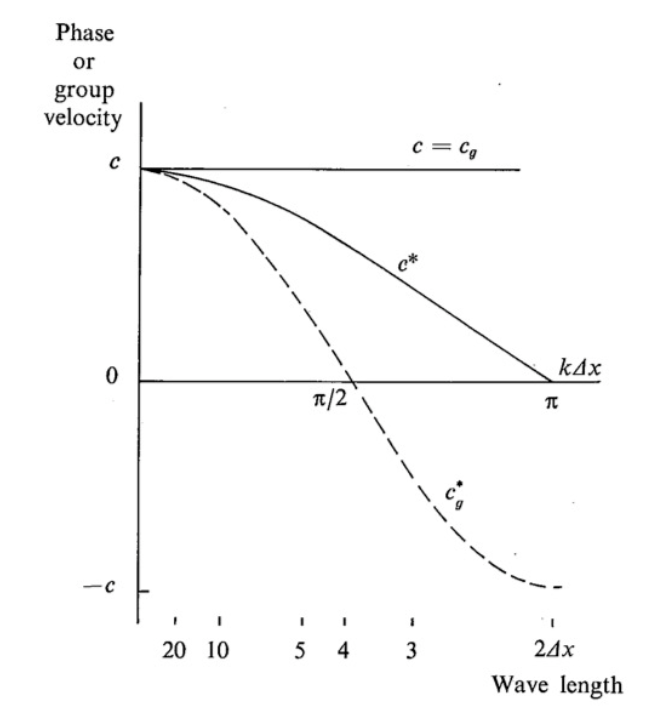
\includegraphics[width=0.45\linewidth]{uploads/Screenshot 2024-11-14 112837.png}
	\caption{Phase speed and group velocity, in the case of the linear advection equation, $c$ and $c_g$, and in the case of the corresponding differential-difference equation with second-order centered space differencing, $c^*$ and $c^*_g$}
	\label{fig:4.2.2}
\end{figure}


Notice: for the exact advection equation \ref{eq:linear adv eq} both individual waves and wave packets, that is, places where superposition of waves results in a maximum amplitude of a group of neighboring wave numbers, propagate at the same constant velocity $c=c_g$. Introduction of the centered space finite difference quotient both makes the phase speed and the group velocity decrease as the wave number increases. The error is particularly great for the shortest resolvable wave lengths; waves with wave lengths less. Than $4\Delta x$ even have a negative group velocity. This means that wave packets made up of these waves propagate in the direction opposite to the advection velocity and opposite to the direction of propagation of individual waves.
Thus, when using such a staggered grid, the phase speed and group velocity diagram shown in \ref{fig:4.2.2} is reduced to its left half, covering waves with wave lengths of up to $4\Delta x$ only. This is a tremendous improvement. If we wish to have waves with wave lengths between $4\Delta x$ and $2\Delta x$ in our calculation we can reduce the grid length by a factor of two and perform a much more accurate integration, using the same amount of computation time than with a grid that is not staggered.
\subsection{Two dimension}
The system of equations for two-dimensional gravity waves is given by:
\begin{align}\label{5.2.5}
	\frac{\partial u}{\partial t}=-g\frac{\partial H}{\partial x}        \\
	\frac{\partial v}{\partial t}=-g\frac{\partial H}{\partial y} \notag \\
	\frac{\partial H}{\partial t}=-H_0\left(\frac{\partial u}{\partial x}+\frac{\partial v}{\partial y}\right)\notag
\end{align}
with $\omega^2=gH_0(k^2+l^2)$ the wave frequency.
With two dimensions and three dependent variables, a large number of spatial arrangements of the variables are possible. For the present we consider the three rectangular arrangements shown below. The identifying letters (A), (E) and (C) are chosen so as to conform with the symbols used by Winninghoff and Arakawa (Arakawa, 1972).
\begin{figure}[htbp]
	\centering
	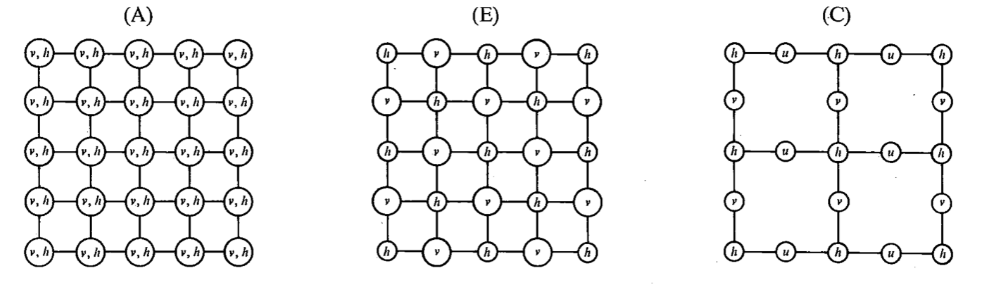
\includegraphics[width=0.5\linewidth]{uploads/Screenshot 2024-11-14 114112.png}
	\caption{Three types of lattice considered for the finite difference solution of \ref{5.2.5}}
	\label{fig:5.2.1}
\end{figure}
Grid arrangements significantly influence the accuracy and efficiency of finite difference solutions. Among the considered grids (A, E, and C), grid (C) offers the most accurate phase speed for gravity waves due to its spatial configuration, but it complicates calculations of Coriolis forces because velocity components are not collocated.
The admissible regions of wave numbers in the wave number plane can be found by considering the shortest resolvable wave lengths. Note that with lattice (E) the lines joining the nearest points with the same variable make an angle of $\frac{\pi}{4}$ with the grid lines while with the other two lattices these lines are along the grid lines.
Grid (E), with its staggered arrangement, provides computational advantages over grid (A), reducing dispersion errors and requiring less computation time while achieving comparable results. However, it is prone to issues with two-grid-interval waves arising from decoupling of subgrids, which can lead to spurious stationary solutions.

Two-grid-interval waves are caused by the decoupling of solutions on (C) subgrids in the (E) lattice. These manifest as spurious stationary waves or low-frequency inertia oscillations. They are triggered by artificial boundary conditions, latent heat release, or orographic forcing. This issue highlights the importance of addressing subgrid interactions in numerical models.

When Coriolis terms are included in the equations:
\begin{align}\label{5.3.4}
	\frac{\partial u}{\partial t}=-g\frac{\partial H}{\partial x}+fv        \\
	\frac{\partial v}{\partial t}=-g\frac{\partial H}{\partial y}-fu \notag \\
	\frac{\partial H}{\partial t}=-H_0\left(\frac{\partial u}{\partial x}+\frac{\partial v}{\partial y}\right)\notag
\end{align}
their inclusion complicates grid selection. Grid (C), ideal for pure gravity waves, struggles with Coriolis terms. Grids (B) and (E) perform similarly but exhibit dispersion issues for the shortest waves. The geostrophic adjustment process, governed by these equations, disperses high-frequency waves until the motion approaches geostrophic balance. Accurate simulation of this process requires careful selection of grid arrangements and numerical methods.

It is not obvious how we should analyse various arrangements of variables. Our primary concern here is to consider \ref{5.3.4} as part of the complete system of primitive equations. We are interested in large-scale motions, otherwise we would not be including the Coriolis terms.

On the large scale, the primitive equations admit two district types of motion : low-frequency, quasi-geostrophic and quasi-nondivergent flow and high-frequency gravity-inertia waves. Gravity-inertia waves are continually excited in the atmosphere. However, as they are dispersive, a local accumulation of wave energy disperses with time. This process is known as geostrophic adjustment; the remaining motion is in approximate geostrophic balance and changes only slowly in time. In this chapter we are concerned with the correct simulation of this process, which is essentially governed by the gravity-inertia wave equations \ref{5.3.4}.

We consider five ways of distributing the dependent variables in space, shown in \ref{fig:5.1.3}. We denote by $d$ the shortest distance between neighbouring points carrying the same dependent variable. In the figure $d$ is the same for each of the five lattices; thus, all the lattices have the same number of dependent variables per unit area. The computation time needed for an integration on each of the lattices will be about the same; the properties of the solution obtained, though, will differ because of the effect of the space arrangement of variables.

Using the subscripts shown in the figure, we define the centered space differencing operator by
\begin{equation}
	\delta_x\alpha=\frac{1}{d'}\left(\alpha_{i+1/2, j}-\alpha_{-1/2,j}\right)
\end{equation}
this rotation is applicable to all the lattices. Here $d'$ is the distance between the points between which the finite difference is taken. Thus, for lattices (A) through (D) $d'$ is equal to the grid size $d$, and for the lattice (E) it is equal to $\sqrt{2d}$.\begin{figure}[h]
	\centering
	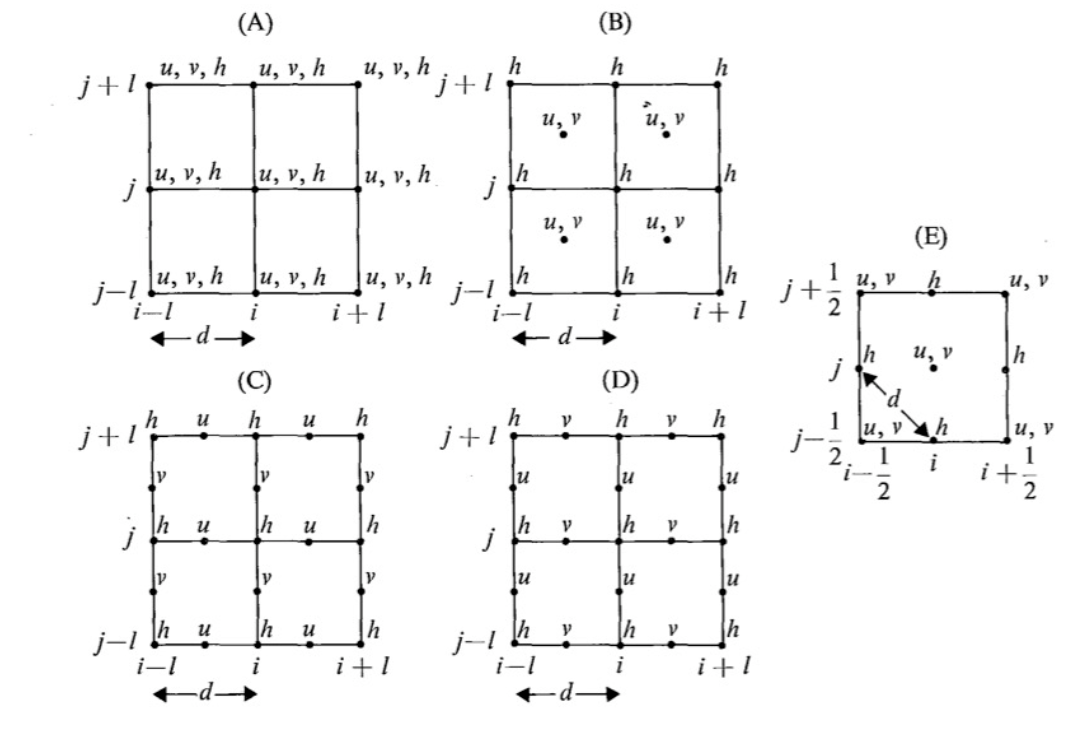
\includegraphics[width=0.5\linewidth]{uploads/Screenshot 2024-11-14 122636.png}
	\caption{Five types of lattice considered for the finite difference solution of \ref{5.3.4}}
	\label{fig:5.3.1}
\end{figure}

The phase speed function,
\begin{equation}\label{5.3.11}
	\left(\frac{\omega}{f}\right)^2=1+\frac{gH}{f^2}k^2
\end{equation}
shows that frequency increases monotonically with wave number, ensuring the group velocity  $\frac{\partial v}{\partial k}$ is never zero. This prevents local wave energy accumulation during geostrophic adjustment. The non-dimensional frequency $\frac{\omega}{f}$ depends on  $kd$ and $\frac{\lambda}{d}$, where the radius of deformation is $$\lambda=\sqrt{\frac{gH}{f}}$$ never equal to zero.


Dissipative numerical schemes can be useful in filtering high-frequency unphysical waves during the geostrophic adjustment process. These schemes prevent excessive wave amplitudes caused by artificial boundary conditions or abrupt grid changes. However, dissipation must be applied selectively to avoid distorting physical processes. For gravity-inertia wave terms, dissipation can accelerate the adjustment process by damping unphysical high-frequency waves. This approach is acceptable when only the final geostrophic state is of interest, but it should be avoided if the high-frequency waves themselves are the focus of study.


Grid (C) provides the closest approximation to the exact solution, avoiding false group velocities, while grids (B) and (E) exhibit issues with false low frequencies and stationary solutions. Grids (D) and (A) have poor dispersion properties and are unsuitable for accurate simulations.

In conclusion, grid (C) is the best choice for simulating geostrophic adjustment due to its superior dispersion properties and minimal spurious wave generation. Staggered grids (B) and (E) are viable alternatives but require methods to address spurious low-frequency waves. Proper dissipation, applied selectively, can enhance numerical stability without compromising physical accuracy.

\begin{figure}[htpb]
	\centering
	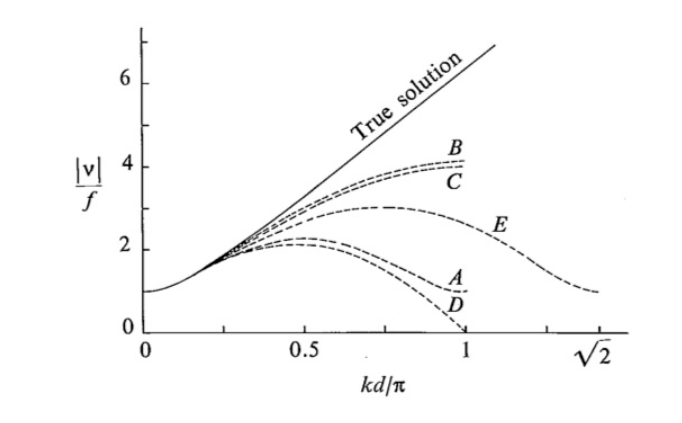
\includegraphics[width=0.5\linewidth]{uploads/Screenshot 2024-11-14 124014.png}
	\caption{The function $\frac{\omega}{f}$ given by \ref{5.3.11}. The wavelength of the shortest resolvable wave along the $x$ axis is $sd$ for lattices (A) through (D), and $\sqrt{2d}$ for the lattice (E). Thus, we have to consider the range $0<kd\leq\pi$ for lattices (A) through (D), and the range $0<kd\leq\sqrt{2\pi}$ for the lattice (E).}
	\label{fig:5.3.2}
\end{figure}


If we consider the one-dimensional case in which the dependent variables are constant along the lines
, we obtain results for these two lattices. In general, we define the coordinate system x’, y’ by rotating the x,y in the positive direction through an angle of $\pi/4$, and then, using some velocity transformations we change from variables $u,v$ to new dependent variables $u',v'$. We find that the dispersion properties of the lattices (B) and (E) can be considered equivalent. A gravity-inertia wave in one of these lattices has phase speed and dispersion properties identical to those of the same wave with its front rotated through an angle of $\pi/4$ in the other lattice.

Considering the two dimensional case, the values of $\frac{\omega}{f}$ that are obtained in the two-dimensional case for the true solution and those using lattices (B) and (C) are shown in \ref{fig:5.3.3}. The diagram for lattice (E) can be obtained by a counterclockwise rotation of the (B) lattice diagram.
\begin{figure}[h]
	\centering
	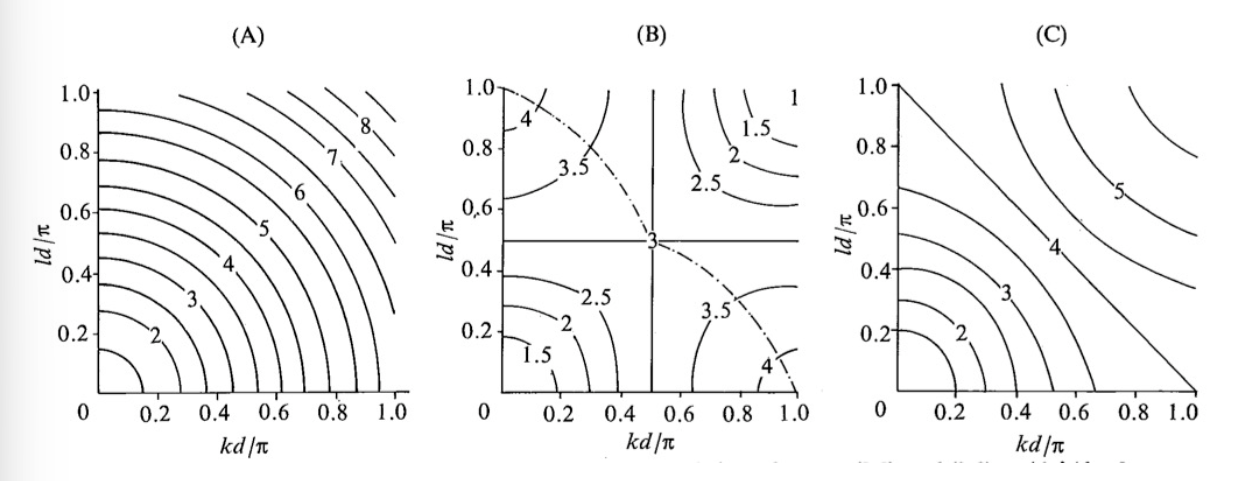
\includegraphics[width=0.5\linewidth]{uploads/Screenshot 2024-11-14 124824.png}
	\caption{The function $\omega/f$ for the true solution}
	\label{fig:5.3.3}
\end{figure}
In the two-dimensional case, lattice (C) provides a significantly better approximation to the exact solution compared to lattices (B) or (E). In the (B) lattice diagram, a dot-dashed line indicates a maximum value of $\omega / f$ for a given ratio $l/f$, but such a feature is absent in both the (C) lattice diagram and the exact solution. This absence highlights the advantage of lattice (C), as it avoids waves with group velocities of the wrong sign. However, the effectiveness of lattice (C) depends on the parameter $\lambda /d$, where $\lambda$ is the radius of deformation. If $\lambda /d$ approaches 1 or less, as might occur in conditions of weak stability, the advantages of lattice (C) diminish. Fortunately, for typical grid sizes in atmospheric models, this is not an issue, leading Arakawa and Lamb (1976) to conclude that lattice (C) is the best choice for simulating geostrophic adjustment processes.

Lattices (B) and (E), on the other hand, struggle with false low frequencies in the shortest waves. Specifically, the two-grid-interval wave, which was stationary as a pure gravity wave, now behaves like a pure inertia oscillation. This issue arises from the decoupling of gravity wave solutions on the two complementary (C)-type subgrids that make up these lattices. Strategies to address these problems are discussed in later sections.


Dissipation in numerical schemes should only be used selectively. For advection, dissipative schemes are generally unnecessary and can lead to energy cascading falsely into short waves. However, short waves may still appear due to boundary reflections, sudden grid changes, or rapidly changing coefficients. In such cases, limited dissipation can help mitigate these effects.

For gravity-inertia waves, dissipation can be helpful in damping high-frequency unphysical waves, speeding up the geostrophic adjustment process. This adjustment relies on wave dispersion, not dissipation, but selective dissipation can approximate the result. If only the final balanced state is important, dissipation is acceptable. However, if high-frequency waves are the focus, dissipation should be avoided to preserve accuracy.
\section{Spectral Methods}\label{sec:spectral method}
Spectral methods are an approach to discretization, the main idea is to express my basic variables in terms of other functions.
In some cases the use of finite differences is a simple and direct method to solve differential equations. However this is not the only method. There are other ways in which one can solve differential equations numerically using a special approach that is based on special functions.
\paragraph{Properties of spectral methods}
\begin{itemize}
	\item Derivative becomes multiplication, i.e. algebraic operations.
	\item Within the limits of the truncation the numerical derivative is exact.
	\item There is no aliasing.
	\item The smallest wavelength in the truncation corresponds to the minimum scale that can be resolved.
\end{itemize}
The main example of this approach is the usage of trigonometric functions within the context of the more general theory of Fourier analysis. Consider the Oscillation equation:
\begin{equation}\label{eq:oscillation}
	\frac{\partial^2\Phi}{\partial t^2}=c^2\frac{\partial^2\Phi}{\partial x^2}
\end{equation}
where $\Phi$ is the deviation from the rest position.
This equation could also express the vibration modes of a string of length L fixed at the extremities. That mathematically is expressed by the fact that the boundary conditions at the extremes are zero. Defining $\Psi$ the unknown variable:
\begin{equation}
	\Phi(x,t)=\Psi(x)e^{i\omega t}
\end{equation}
with $e^{i\omega t}=\cos \omega t+i\sin\omega t$
also
\begin{equation}
	\frac{\partial^2\Psi}{\partial x^2}+k^2\Psi=0
\end{equation} with $k=\frac{\omega}{c}$
The solution is either $$\Psi(x)=A\sin(kx+\delta)$$
or $$\Psi(x)=A\cos(kx+\delta)$$
The boundary conditions for fixed extremities ($\Psi(0)=\Psi(L)=0$) exclude the cosine solution, so the general solution is
\begin{equation}\label{psin}
	\Psi_n(x)=A_n\sin{nk x}
\end{equation}
this is not the only one function: I'll have an integer number of wavefunctions that satisfy this condition meaning that $k$ cannot be arbitrary, i.e. the boundary conditions are satisfied only for integer values of $k$
$$k=\frac{\pi}{L}, \frac{2\pi}{L}, \dots, \frac{n\pi}{L}$$
(only $\sin$ functions that have an integer number of cycles can be a solution.)  We'll get infinite number of solutions that satisfy the boundary conditions. These are known as eigenfunctions (or vectors) $\Psi_n(x)$ of the wave equation for the string, and they are linear transformations acting on finite vector (they are of the same number as the dimension of the matrix). The most important property of the eigenfunction is the \textbf{orthogonality}:
\begin{equation}
	\int_0^L\Psi_n(x)\Psi_m(x)dx=C_n\delta_{nm}
\end{equation}
with $$\delta_{mn}=\begin{cases}
		1 , & \text{if $n=m$}    \\
		0,  & \text{if $n\ne m$}
	\end{cases}$$
The eigenfunctions can always be normalized so that the constants C becomes 1. It is easy to show that in this case the normalized eigenfunctions are:
\begin{equation}
	\Psi_n(x)=\sqrt{\frac{2}{L}}\sin\frac{n\pi x}{L}
\end{equation}
The most important property of the eigenfunction is the
orthogonality, in fact:
For $n=m$:
$$\int_0^L\sin^2\frac{n\pi x}{L}dx=\frac{1}{2}\int_0^L\left[1-\cos\frac{2n\pi x}{L}\right]dx=\frac{x}{2}\bigg|_0^L-\frac{L}{4\pi n}\sin\frac{2n\pi x}{L}\bigg|_0^L=\frac{L}{2}$$
for $n\ne m$:
\begin{equation*}
	\begin{split}
		\int_0^L\sin\frac{n\pi x}{L}\sin\frac{m\pi x}{L}dx=\frac{1}{2}\int_0^L\left[\cos\frac{(n-m)\pi x}{L}-\cos\frac{(n+m)\pi x}{L}\right]dx= \\
		=\frac{1}{2}\frac{L}{n-m}\sin\frac{(n-m)\pi x}{L}\bigg|_0^L-\frac{1}{2}\frac{L}{n+m}\sin\frac{(n+m)\pi x}{L}\bigg|_0^L=0
	\end{split}
\end{equation*}
The orthogonality can be used to describe every function $f(x)$, meaning that I can generalize the concept managing to write functions as sum of eigenfunctions:
$$f(x)=\displaystyle\sum_na_n\Psi_n(x)$$
How can I find the coefficients? Multiply both sides by another
eigenfunction $\Psi_k(x)$ and integrate:
$$\int_0^Lf(x)\Psi_k(x)dx=\displaystyle\sum_na_n\int_0^L\Psi_n(x)\Psi_k(x)dx=\displaystyle\sum_na_n\delta_{kn}=a_n$$
so it seems that every function can be expressed as a sum of countable terms. This sum is over integer index, $f(x)$ is continuous. I should find out its behavior in every point, this can be described by a slighter lower order of infinity.
\paragraph{Fourier theory} Every function can be expressed in a set of eigenfunction, expanded over a series of the trigonometric functions.
\begin{equation}
	f(x)\approx A_0+\displaystyle\sum_{k=1}^nA_k\cos kx+\sum_{k=1}^nB_n\sin kx
\end{equation}
where the A's and B's are computed from orthogonality relations as we've seen before.
\begin{align*}
	A_0=\frac{1}{2\pi}\int_{-\pi}^{\pi}f(x)dx           \\
	A_{\pi}=\frac{1}{\pi}\int_{-\pi}^{\pi}f(x)\cos kxdx \\
	B_{\pi}=\frac{1}{\pi}\int_{-\pi}^{\pi} f(x)\sin kx dx
\end{align*}

We have already seen the importance of Euler formula $e^{i\theta}=\cos\theta+i\sin\theta$, it is useful to see the form of the Fourier series in terms of the complex exponential, substituting the expression for the coefficients in the un-truncated representation of $f(x)$.
\begin{equation}\label{eq.complex Fourier}
	f(x)=\displaystyle\sum_{k=-\infty}^{+\infty}c_ke^{ikx}
\end{equation}
with
\begin{equation}
	c_k=\frac{1}{2\pi}\int f(\xi)e^{-ik\xi}d\xi
\end{equation}
This approximation works fine if everything is smoothed, but if there are jumps it increases amplitude over them, this is known as Gibbs phenomenon.
The Gibbs phenomenon happens when we use a Fourier series to represent a function with a sudden jump (discontinuity). Near the jump, the Fourier series creates wavy overshoots and undershoots. As we add more terms to the series, the first overshoot stays at about 9\% of the jump size, and the waves don’t completely go away. Instead, they get squeezed closer to the jump, so their overall effect becomes smaller, and the total area of the waves approaches zero.
\begin{figure}
	\centering
	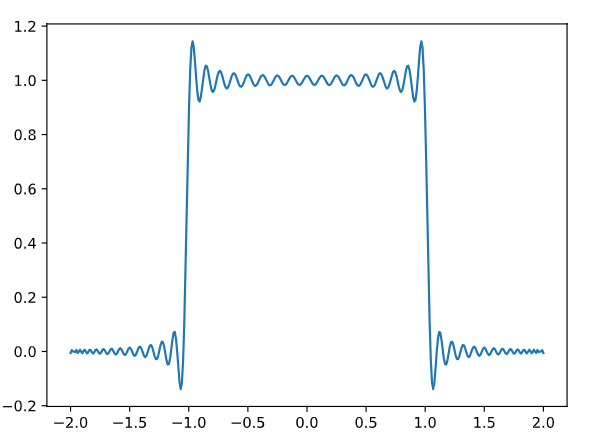
\includegraphics[width=0.5\linewidth]{uploads/Screenshot 2024-11-14 170405.png}
	\caption{Representation of Gibbs phenomenon.}
	\label{fig:Gibbs}
\end{figure}
At the jump point, the Fourier series gives the average of the function's both side limits toward the point.

This new representation of functions has some problems, even though manages to solve problems with higher order: accuracy. The eigenfunction expansion, the Fourier series, allows us to find a new representation of functions. What we have found is an alternative but equivalent representation of a function that has all the same properties of the original function. The question now arise if we can use these alternative form to find a way to drive a numerical solution that is somewhat better or cheaper or easier.. Applying this into a set of ordinary equations, let's for instance take the advection equation:
$$ \frac{\partial u}{\partial t}=-c\frac{\partial u}{\partial x} $$
and let's use a Fourier representation using the first $N$ components:
\begin{equation}\label{eq.u(x)}
	u(x)=\displaystyle\sum_{k=1}^Nu_k(t)e^{ikx}
\end{equation} with the initial condition:
\begin{equation}\label{eq.u(x,0)}
	u(x,0)=\displaystyle\sum_{k=1}^Nu_k(0)e^{ikx}
\end{equation}
now substituting, multiplying by $e^{jkx}$ and integrating  over $x$, with $$\int e^{ikx}e^{ijx}dx=\delta_{ij}$$
We get back exactly, in the linear case
\begin{equation}
	\frac{du_k}{dt}=-cku_k(t)
\end{equation}

\subsection{Numerical spectral solution (nonlinear)}
Consider now the nonlinear advection equation:
\begin{equation}
	\frac{\partial u}{\partial t}=-u\frac{\partial u}{\partial x}
\end{equation}
Let's try a spectral solution substituting eq.\ref{eq.u(x)} and eq.\ref{eq.u(x,0)},
\[
	\sum_k \frac{d}{dt} u_k(t) e^{ikx} = -\sum_j u_j(t) e^{ijx}
	\sum_k \frac{d}{dx} u_k(t) e^{ikx} = -\sum_{k,j} ik u_j(t) u_k(t) e^{ijx} e^{ikx}
\]
projecting on another eigenfunction and integrating:
\[
	\int \sum_k \frac{du_k}{dt} e^{ikx} e^{inx} \, dx =
	- \int \sum_{k,j} ik \, u_j(t) u_k(t) e^{ijx} e^{ikx} e^{inx} \, dx
\]
the integrals yield:
\begin{align*}
	\int e^{ikx}e^{inx}dx=\delta_{kn} \\
	\int e^{ikx}e^{ikx}e^{inx}dx=c_{ikn}
\end{align*}
so the spectral system looks like
\begin{equation}\label{eq.spectral system nonlinear}
	\frac{du_k}{dt}=-\displaystyle\sum_{j,n}iku_j(t)u_k(t)c_{kjn}
\end{equation}
These are now nonlinear ordinary differential equation and we to compute the $c_{kjn}$ coefficients, also known as \textit{interaction coefficients}. The equations are not clearly separated, every spectral component is depending on its evolution on every other component $u_j$.
The interaction coefficients are defined as:
\begin{equation}
	c_{knj}=\delta_{k,j+n}=\begin{cases}
		1, & \text{if $k=j+n$} \\
		0, & \text{otherwise}
	\end{cases}
\end{equation}
The method is very convenient and it has a lot of good properties ( by the way,
quadratic properties are conserved, within the truncation limit). However the
number of coefficients grows very rapidly with the truncation limit as $N^3$.
Furthermore, every particular non linear term will generate its own set of
interaction coefficients, so there will be many set of c’s to compute and store.
These days a typical climate model will have truncation of the order of $100$, so
for each term $10^6$ coefficient will have to be computed.

\section{Spherical frame}\label{Sec:models on the sphere}
\begin{center}
	\textit{The following section refers to the slides of prof.Navarra and his discussion, in the book this topic is faced differently.}
\end{center}
We will use the shallow water equation, but in order to have a realistic case, we need to put it on the sphere. We start from the usual equation of the homogeneous flow, also known as shallow water equation on the sphere. For convenience we introduce the geopotential $\Phi= gH$, representing the gravitational potential energy per unit mass related to height in the atmosphere.
\begin{align}
	\frac{\partial u}{\partial t}=-u\frac{\partial u}{\partial x}-v\frac{\partial u}{\partial y}+fv-\frac{\partial\Phi}{\partial x} \\
	\frac{\partial v}{\partial t}=-u\frac{\partial v}{\partial x}-v\frac{\partial v}{\partial y}-fu-\frac{\partial\Phi}{\partial y} \\
	\frac{\partial\Phi}{\partial t}=-\frac{\partial}{\partial x}u\Phi-\frac{\partial}{\partial y}v\Phi
\end{align}
Let's now consider the momentum equation and equation of continuity in vector form. Using a spherical rather than a $(x,y)$ grid, $u$ and $v$ become longitudinal and latitudinal components of wind. It is convenient to use the representation of scalar fields on the globe, so  write velocities $U=u\cos\phi$ and $V=v\cos\phi$ in terms of the latitude $\phi$, so we can write the system in vector form using the horizontal wind $\vec{V}=iU+jV$ ($i$ is the longitude component east-west, while $j$ is the latitudinal north-south):
\begin{align}\label{eq.partialV}
	\frac{\partial\vec{V}}{\partial t}+(\vec{V}\cdot\nabla)\vec{V}=-f\vec{k}\times\vec{V}-\nabla\Phi \\
	\frac{\partial\Phi}{\partial t}+(\vec{V}\cdot\nabla)\Phi=-\Phi\nabla\cdot\vec{V}\notag
\end{align}
$\vec{k}$ is the vertical component. In the geopotential equation, $(\vec{V}\cdot\nabla)\Phi$ is the advection term at the geopotential, while the right side of the equation represents the divergence.
Using the identity
$$(\vec{V}\cdot\nabla)\vec{V}=\nabla\left(\frac{\vec{V}\cdot\vec{V}}{2}\right)+\zeta\vec{k}\times\vec{V}$$
that allows us to modify non-linearity of the advection $(\vec{V}\cdot\nabla)\vec{V}$ , we can re-write the first equation of \ref{eq.partialV} as
\begin{equation}\label{eq.V}
	\frac{\partial\vec{V}}{\partial t}=-(\zeta+f)\vec{k}\times\vec{V}-\nabla\left(\Phi+\frac{\vec{V}\cdot\vec{V}}{2}\right)
\end{equation}


On the left we have the tendency (rate of change of velocities); on the right:
\begin{enumerate}
	\item the changes in advection in zonal components is actually driven by vorticity and $f$ (Coriolis) coupled with meridional motion.
	\item the rate of geopotential generating tendency to the currents. Different gradients in the speed will generate acceleration or deceleration according to the gradient of the current, this term is coming from the advection. The advection is operating with vorticity in a cross way, also kinetic energy $(\vec{V}\cdot\vec{V})$ is operating.
\end{enumerate}


Using the definitions of vorticity (curl of the velocity field) and divergence (divergence of the velocity field). Vorticity $\zeta$ represents the rotational or swirling motion of the fluid, while the divergence $D$ represents the expansion or contraction of the fluid, i.e. the rate at which the fluid is spreading out or converging.
\begin{align}\label{eq.defsvortdiv}
	\zeta=\vec{k}\cdot(\nabla\times \vec{V}) \\
	D=\nabla\cdot\vec{V}
\end{align}
We can then find the expressions for the time rate change of vorticity and divergence:
\begin{equation}\label{eq.for vorticity time change}
	\frac{\partial\zeta}{\partial t}=-\nabla\cdot(\zeta +f)\vec{V}
\end{equation}
because, from the definition and the eq.\ref{eq.V}, the geopotential and kinetic term goes to zero as the curl of the gradient is zero. In this equation $\zeta$ is the relative vorticity, while $f$ is the planetary vorticity. And for the divergence we find:
\begin{equation}\label{eq.for divergence time change}
	\frac{\partial D}{\partial t}=\vec{k}\cdot\nabla\times(\zeta+f)\vec{V}-\nabla^2\left(\Phi+\frac{\vec{V}\cdot\vec{V}}{2}\right)
\end{equation}
It is also useful to divide the geopotential from its global constant mean, $\bar{\Phi}$, $\Phi=\bar{\Phi}-\Phi'$, the continuity equation becomes:
$$\frac{\partial\Phi'}{\partial t}=\frac{\partial\Phi}{\partial t}=-(\vec{V}\cdot\nabla)(\bar{\Phi}+\Phi')-(\bar{\Phi}-\Phi')D=-[\vec{V}\cdot\nabla\Phi'+\Phi'D]-\bar{\Phi}D=-\nabla\cdot\Phi'\vec{V}-\bar{\Phi}D$$
The advection will kill the mean, so we'll have only its action on the deviation.

\paragraph{Why decompose using vorticity and divergence?}
By separating the rotational (vorticity) and compressional (divergence) components, you can better understand the dynamics of the flow field, such as areas dominated by rotation (e.g., cyclones, anticyclones) or regions of convergence or divergence (e.g., updrafts, downdrafts).
In meteorology and oceanography, the large-scale velocity field is often approximated using vorticity ($\zeta$) and divergence ($D$) because these quantities are central to the equations of motion, making them more directly tied to the dynamics than $\vec{V}$ itself.


Any vector field (like $\vec{V}$) also can be decomposed into two components using Helmholtz theorem:
\begin{itemize}
	\item Irrotational (divergence-driven) derived from a scalar potential $\chi$
	\item Solenoidal (vorticity-driven) derived from a streamfunction $\psi$
\end{itemize}
The idea is starting from the velocity field $\vec{V}$, getting the vorticity and divergence equations, solve for the streamfunction $\psi$ and the scalar velocity potential $\chi$ using $\zeta$ and $D$ (see below), and reconstruct the velocity field using Helmholtz theorem.
\subsection{The Helmholtz theorem}
Helmholtz showed that any vector field tangent to the surface of a sphere can be
split in terms of two scalar functions, one rotational (velocity) and another nonrotational (divergence), in the following way:
\begin{equation}\label{eq.helmholtz}
	\vec{V}=\vec{k}\times\nabla\psi+\nabla\chi
\end{equation}
where $\vec{k}$ is the vector normal to the surface of the sphere.
\begin{itemize}
	\item The \textbf{streamfunction} is a scalar function used to describe two-dimensional (or axisymmetric three-dimensional) incompressible flow. It simplifies the analysis of fluid motion by providing a way to represent the velocity field such that the incompressibility condition is automatically satisfied. It describes the rotational part of the flow.
\end{itemize}

By the definitions \ref{eq.defsvortdiv}, we can write through the Helmholtz theorem:
\begin{equation}\label{eq. vorticity}
	\zeta=\nabla^2\psi
\end{equation}
\begin{equation}\label{eq.divergence}
	D=\nabla^2\chi
\end{equation}
We could also derive these definitions from the description of $D$ and $\zeta$ in spherical coordinates:
\begin{align*}
	D=\frac{1}{a\cos\phi}\left(\frac{\partial u}{\partial\lambda}+\frac{\partial v\cos\phi}{\partial\phi}\right)=\frac{1}{a\cos^2\phi}\left(\frac{\partial U}{\partial\lambda}+\cos\phi\frac{\partial V}{\partial\phi}\right) \\
	\zeta= \frac{1}{a\cos\phi}\left(\frac{\partial v}{\partial\lambda}-\frac{\partial u\cos\phi}{\partial\phi}\right)=\frac{1}{a\cos^2\phi}\left(\frac{\partial V}{\partial\lambda}-\cos\phi\frac{\partial V}{\partial\phi}\right)
\end{align*}
using the expression for $U$ and $V$, for instance in the divergence:
\begin{equation}\label{eq.finitedivergence}
	D=\frac{1}{a\cos^2\phi}\left(\frac{\partial^2\chi}{\partial\lambda^2}+\cos\phi\frac{\partial}{\partial\phi}\left(\cos\phi\frac{\partial\chi}{\partial\phi}\right)\right)=\nabla^2\chi
\end{equation}
so we find that also on the sphere:
\begin{equation}\label{eq. vorticity}
	\zeta=\nabla^2\psi
\end{equation}
and
\begin{equation}\label{eq.divergence}
	D=\nabla^2\chi
\end{equation}

Because of Helmholtz theorem we can write the components in terms of $\psi$ and $\chi$ as:
\begin{align}\label{eq.components helmholtz}
	U=-\frac{\cos\phi}{a}\frac{\partial\psi}{\partial\phi}+\frac{1}{a}\frac{\partial\chi}{\partial\lambda} \\
	V=\frac{\cos\phi}{a}\frac{\partial\chi}{\partial\phi}+\frac{1}{a}\frac{\partial\psi}{\partial\lambda}
\end{align}
And we can find equations for vorticity and divergence rates depending on these new scalar fields, from \ref{eq.for vorticity time change} and \ref{eq.for divergence time change}:
\begin{align}\label{eq.motionforstreamf}
	\frac{\partial}{\partial t}(\nabla^2\psi)=-\frac{1}{a\cos^2\phi}\left[\frac{\partial}{\partial\lambda}(U\nabla^2\psi)+\cos\phi\frac{\partial}{\partial\phi}(V\nabla^2\psi)\right]-2\Omega\left(\sin\phi\nabla^2\chi+\frac{V}{a}\right) \\
	\frac{\partial}{\partial t}(\nabla^2\chi)=+\frac{1}{a\cos^2\phi}\left[\frac{\partial}{\partial\lambda}(V\nabla^2\psi)-\cos\phi\frac{\partial}{\partial\phi}(U\nabla^2\psi)\right]+2\Omega\left(\sin\phi\nabla^2\psi-\frac{U}{a}\right)-\nabla^2\left(\frac{U^2+V^2}{2\cos^2\phi}+\Phi'\right)
\end{align}
together with:
\begin{equation}\label{eq.geostream}
	\frac{\partial\Phi'}{\partial t}=-\frac{1}{a\cos^2\phi}\left[\frac{\partial}{\partial\lambda}(U\Phi')+\cos\phi\frac{\partial}{\partial\phi}(V\Phi')\right]-\overline{\Phi}D
\end{equation}
make the system complete and the three equations above are three prediction equations for the three unknown variables $\psi$, $\chi$ and $\Phi'$. The systems of equations is more complex than the straightforward use of $u$, $v$ and $h$, but $\psi$ and $\chi$ fields are scalar functions that can be expressed easily as spherical harmonics.
The transform technique allows for relatively simple means of solving the equations. The essence of this technique is to transform from spectral space quantities to grid point space quantities, then perform nonlinear products at each grid point, and to reverse quantities from grid point quantities back to spectral quantities. The problems in fact are the nonlinearity terms present in the equations, such as:
$$U\nabla^2\psi,\quad V\nabla^2\psi,\quad U\Phi',\quad V\Phi'\quad \text{and}\quad (U^2+V^2)/2$$

In order to do this, the fields of $\psi$, $\chi$ and $\Phi'$ have to be represented as truncated series of spherical harmonics, as described in the next section.



\subsection{Spherical Harmonics}
The Laplacian in spherical coordinates gives rise to Laplace equation: eq.\ref{eq.finitedivergence}=0, setting it up as a search for the eigenfunctions/eigenvalues requires to solve a Poisson equation with periodic boundary conditions in longitude and zero at the poles.
\begin{equation}\label{eq.sphericalhar}
	\frac{1}{a\cos^2\phi}\left(\frac{\partial^2Y}{\partial\lambda^2}+\cos\phi\frac{\partial}{\partial\phi}\left(\cos\phi\frac{\partial Y}{\partial\phi}\right)\right)=\sigma Y
\end{equation}
the solution can be found for discrete values of two indices $(m,l)$.
The boundary conditions, as in the case of the string, force solution only for
discrete set of values. Because the equation is in two dimension there will
be two families of functions, labeled by the the indices $(l,m)$:
\begin{equation}
	Y_l^m=P_l^m(\sin\phi)e^{im\lambda}
\end{equation}
We can see how we can derive the spherical harmonics by noticing that we can look for solutions of the Laplace equation as $Y=P(\phi)Q(\lambda)$, then
$$\frac{\partial^2P(\phi)Q(\lambda)}{\partial\lambda^2}+\cos\phi\frac{\partial}{\partial\phi}\left(\cos\phi\frac{\partial P(\phi)Q(\lambda)}{\partial\phi}\right)=\sigma a\cos^2\phi P(\phi)Q(\lambda)$$


The two parts are separated in variables so a solution exist
only if they are equal to some constant:
$$\frac{1}{Q}\frac{\partial^2Q(\lambda)}{\partial\lambda^2}=-m^2$$
$$\frac{1}{P(\phi)}\cos\phi\frac{\partial}{\partial\phi}\left(\cos\phi\frac{\partial P(\phi)}{\partial\phi}\right)-\sigma a\cos^2\phi=m^2$$

The periodic boundary condition on longitude require $m$ to be real and discrete, so the solution to the $Q$ equation are longitudinal waves $e^{\pm im\lambda}$. The regularity conditions at the poles (essentially conditions for the solutions to be well-behaved) requires that $\sigma$ be of the form $l(l+1)$ with $l\geq|m|$. Then a change of variables $(u=\sin\phi)$ will put the $P$ equation in the form of the associated Legendre equation whose solutions are the associated Legendre polynomials $P_l^m(\sin\phi)$:
\begin{equation}\label{eq.Legendre polyn}
	P_l^m(\sin\phi)=(1-\sin^2\phi)^{m/2}\frac{d^m}{d(\sin\phi)^m}P_l(\sin\phi)
\end{equation}
where the $P_l(\sin\phi)$ are the Legendre polynomials. For $m=0$, the associated Legendre polynomials reduce to the
Legendre polynomials, the first few associated Legendre
polynomials with $m>0$ are
\begin{align*}
	P_1^1(\sin\phi)=(1-\sin^2\phi)^{1/2}          \\
	P_2^1(\sin\phi)=3\sin\phi(1-\sin^2\phi)^{1/2} \\
	P_2^2(\sin\phi)=3(1-\sin^2\phi)
\end{align*}
they are an orthogonal in variable $\phi$, and the full spherical harmonics are orthogonal in both indices:
\begin{equation}
	Y_l^m=P_l^m(\sin\phi)e^{im\lambda}
\end{equation}
they are an orthogonal system, with respect both indices, so
\begin{equation}
	\int_{-\pi/2}^{\pi/2}\cos\phi d\phi\int_0^{2\pi}Y_l^m(\phi,\lambda)\bar{Y}_i^j(\phi,\lambda)d\lambda=\delta_{mj}\delta_{ij}
\end{equation}
with the normalization:
$$Y_l^m=\sqrt{\frac{2l+1}{4\pi}\frac{(l-m)!}{(l+m)!}}P_l^m(\sin\phi)e^{im\lambda}$$
\begin{figure}[h]
	\centering
	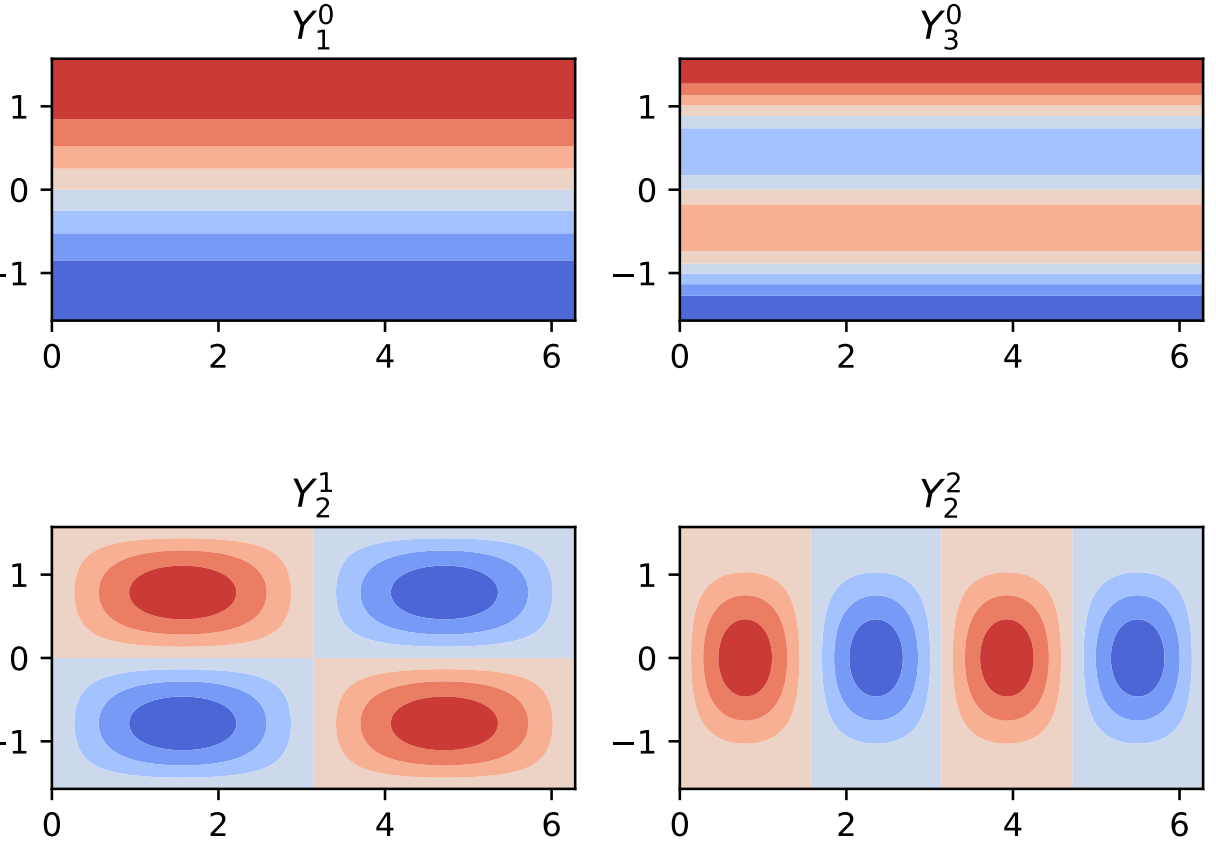
\includegraphics[width=0.5\linewidth]{uploads/Screenshot 2024-11-17 201945.png}
	\caption{Spherical harmonics}
	\label{fig:spherical harmonics}
\end{figure}
There are useful recursion relation for associated Legendre
polynomial and for the spherical harmonics
$$\epsilon_{l+1}^mP_{l+1}^m=\sin\phi P^m_l-\epsilon_l^mP^m_{l-1}$$
and
\begin{equation}\label{eq.A}
	(1-\sin^2\phi)\frac{d}{d(\sin\phi)}Y_l^m=-l\epsilon_{l+1}^mY_{l+1}^m+(l+1)\epsilon_l^mY_{l-1}^m
\end{equation}
with
$$\epsilon_l^m=\left(\frac{(l^2-m^2)}{(4l^2-1)}\right)^{1/2}$$
Note that the relation \ref{eq.A} is effectively transforming the derivation of a spherical harmonics into a difference of other harmonics.



\subsection{Spectral Transforms}
Having now a set of functions that are eigenfunctions of the Laplacian on the sphere is then natural that we look for representations of the physical variables as an expansion in terms of spherical harmonics.

\begin{figure}[htpb]
	\centering
	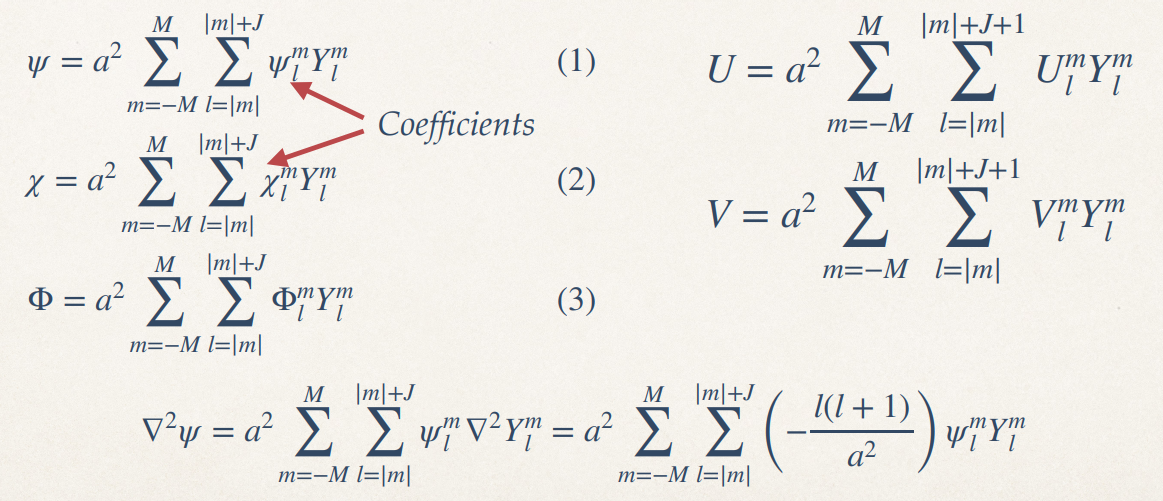
\includegraphics[width=0.5\linewidth]{uploads/Screenshot 2024-11-17 203102.png}
	\caption{spectral representations}
	\label{fig:enter-label}
\end{figure}
Horizontal wind components will have a similar expansion. The expansion for $U$ and for $V$ have an extra component as they are derived from stream function and velocity potential We can use the recurrence formulas of the spherical harmonics to find that
$$\epsilon_{l+1}^mP_{l+1}^m=\sin\phi P^m_l-\epsilon_l^mP^m_{l-1}$$
and
\begin{align*}
	U_l^m=(l-1)\epsilon_l^m\psi^m_{l-1}-(l+2)\epsilon_{l+1}^m\psi_{l+1}^m+im\chi_l^m \\
	V_l^m=-(l-1)\epsilon_l^m\chi_{l-1}^m+(l+2)\epsilon_{l+1}^m\chi_{l+1}^m+im\psi_l^m
\end{align*}
with $\epsilon_l^m$ defined as before.
These expression must be inserted into the equation to obtain ordinary equations for the spherical harmonics coefficients.





Recalling the equation of motion in terms of vorticity and divergence \ref{eq.motionforstreamf} and \ref{eq.geostream}, the linear terms will transform in linear terms for the spherical coefficients, and the laplacians will also be easily done by the multiplication by the eigenvalues. We will need to treat the nonlinear terms $U\nabla^2\psi$, $V\nabla^2\psi$, $U\Phi'$, $V\Phi'$, $(U^2+V^2)/2$.  However, we don't really need all the details of these non linear terms, we only need the total impact on the tendency. In this case, we need only the spectral coefficient of $A(\psi,\chi)$, $B(\psi,\chi)$, $C(\psi,\chi)$ and $E(\psi,\chi)$ non linear terms of the equation of motion. With the spectral coefficient of the non linear terms, we can discretize in time by choosing a time scheme, for example the leap-frog scheme.
\begin{figure}[htpb]
	\centering
	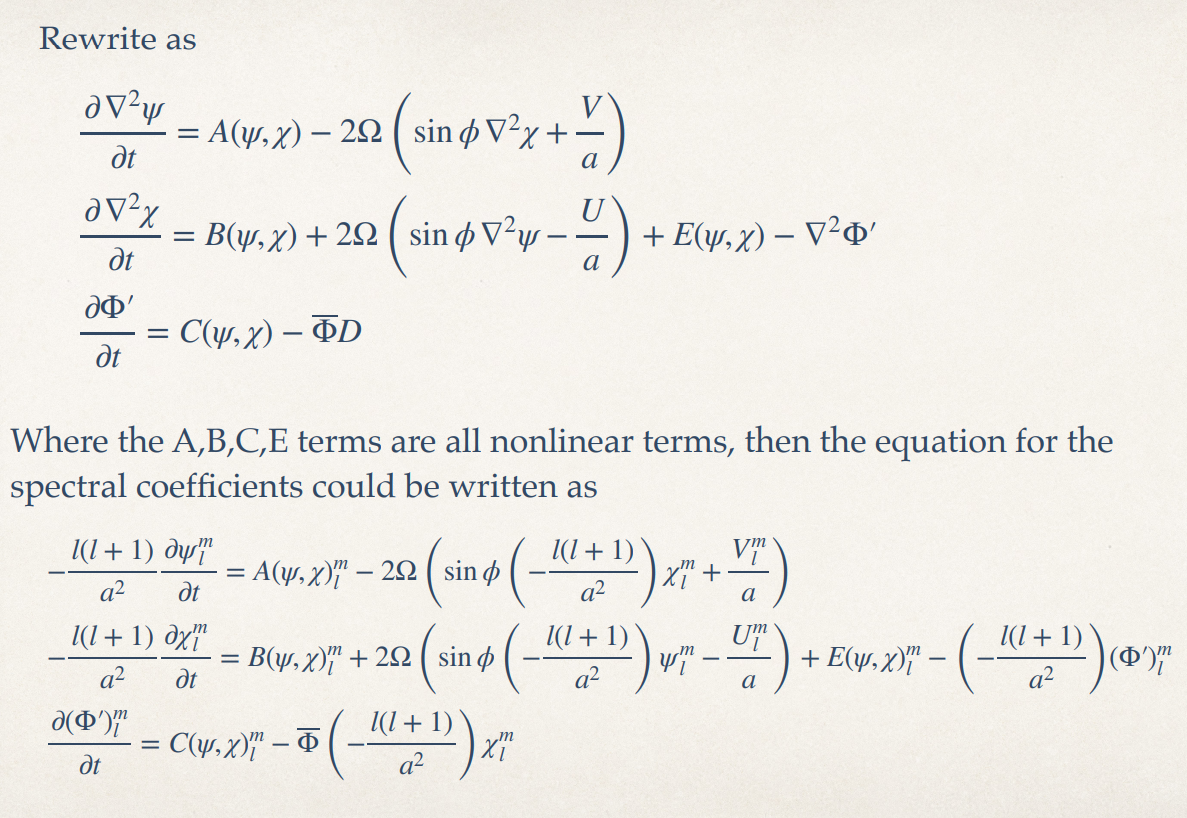
\includegraphics[width=0.5\linewidth]{uploads/Screenshot 2024-11-18 095232.png}\quad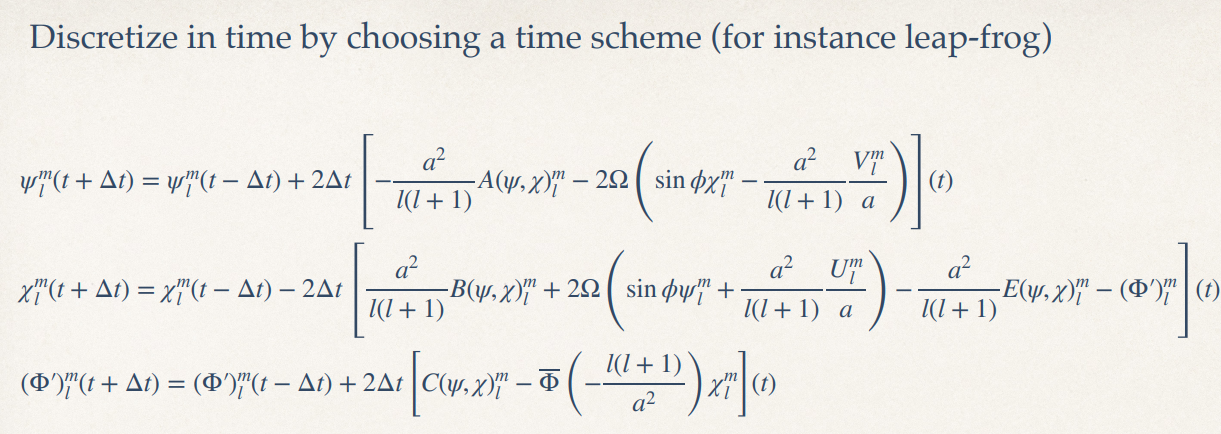
\includegraphics[width=0.5\linewidth]{uploads/Screenshot 2024-11-18 095428.png}
	\caption{Treating nonlinearity with a time discretization with Leap-Frog scheme}
	\label{fig:trating nonlinearity}
\end{figure}

The problem is to find a method to obtain the spectral coefficients of the nonlinear terms. In general the spectral coefficients can be obtained in a similar way to the
Fourier coefficients, projecting on a specific harmonic $Y_k^j$ and integrating.
\[\int_{-\pi/2}^{\pi/2}\cos\phi d\phi\int_0^{2\pi}d\lambda\Psi(\phi,\lambda) Y_k^j(\phi,\lambda)=\int_{-\pi/2}^{\pi/2}\cos\phi d\phi\int_0^{2\pi}d\lambda\displaystyle\sum_{m=-J}^J\displaystyle\sum_{l=|m|}^{|m|+J}\Psi_l^m\delta_{kl}\delta_{mj}=\Psi_k^j\]
so the coefficients can be obtained by integrating the original (physical space) functions with the harmonics. The integration can separated:
\begin{equation}
	\Psi_k^j=\int_{-\pi/2}^{\pi/2}\cos\phi P_k^j(\sin\phi)d\phi\int_0^{2\pi}\Psi(\phi, \lambda)e^{ij\lambda}d\lambda
\end{equation}
where the first integral is the \textit{polynomial integration}. The second is for the \textit{Fourier transform} with dependency on the latitude, so must be done at every latitude over longitude, the result of this Fourier integration is a vector of numbers at any latitude, this is used to make the longitudinal integration and you obtain the coefficients.

\begin{figure}[htpb]
	\centering
	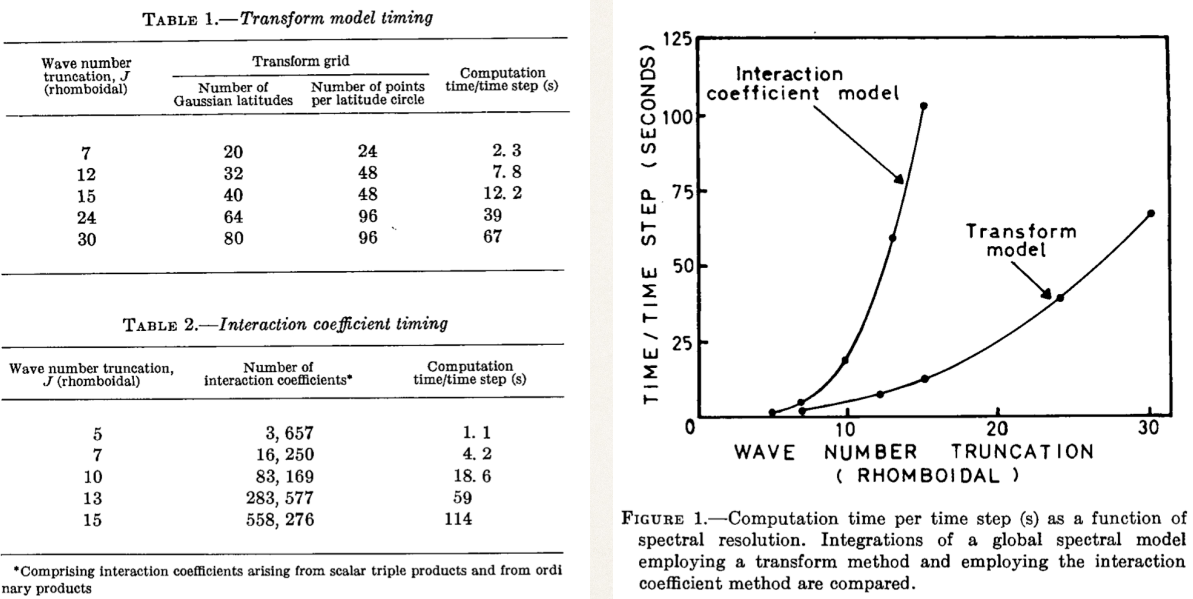
\includegraphics[width=0.58\linewidth]{uploads/Screenshot 2024-11-18 100538.png}
	\caption{Gaussian grids}
	\label{fig:gaussian grids}
\end{figure}

Numerically an integration is a summation, just like the derivatives are differences. However, we have freedom to choose the points and it can be shown that if the points are chosen in special points then the summation for polynomials is exact if enough points are selected. In the case of our models the integration is over latitudes, so we have to choose certain latitudes, these are known as \textit{Gaussian Latitudes}. The minimum number of points is a function of truncation order.

\begin{figure}[htpb]
	\centering
	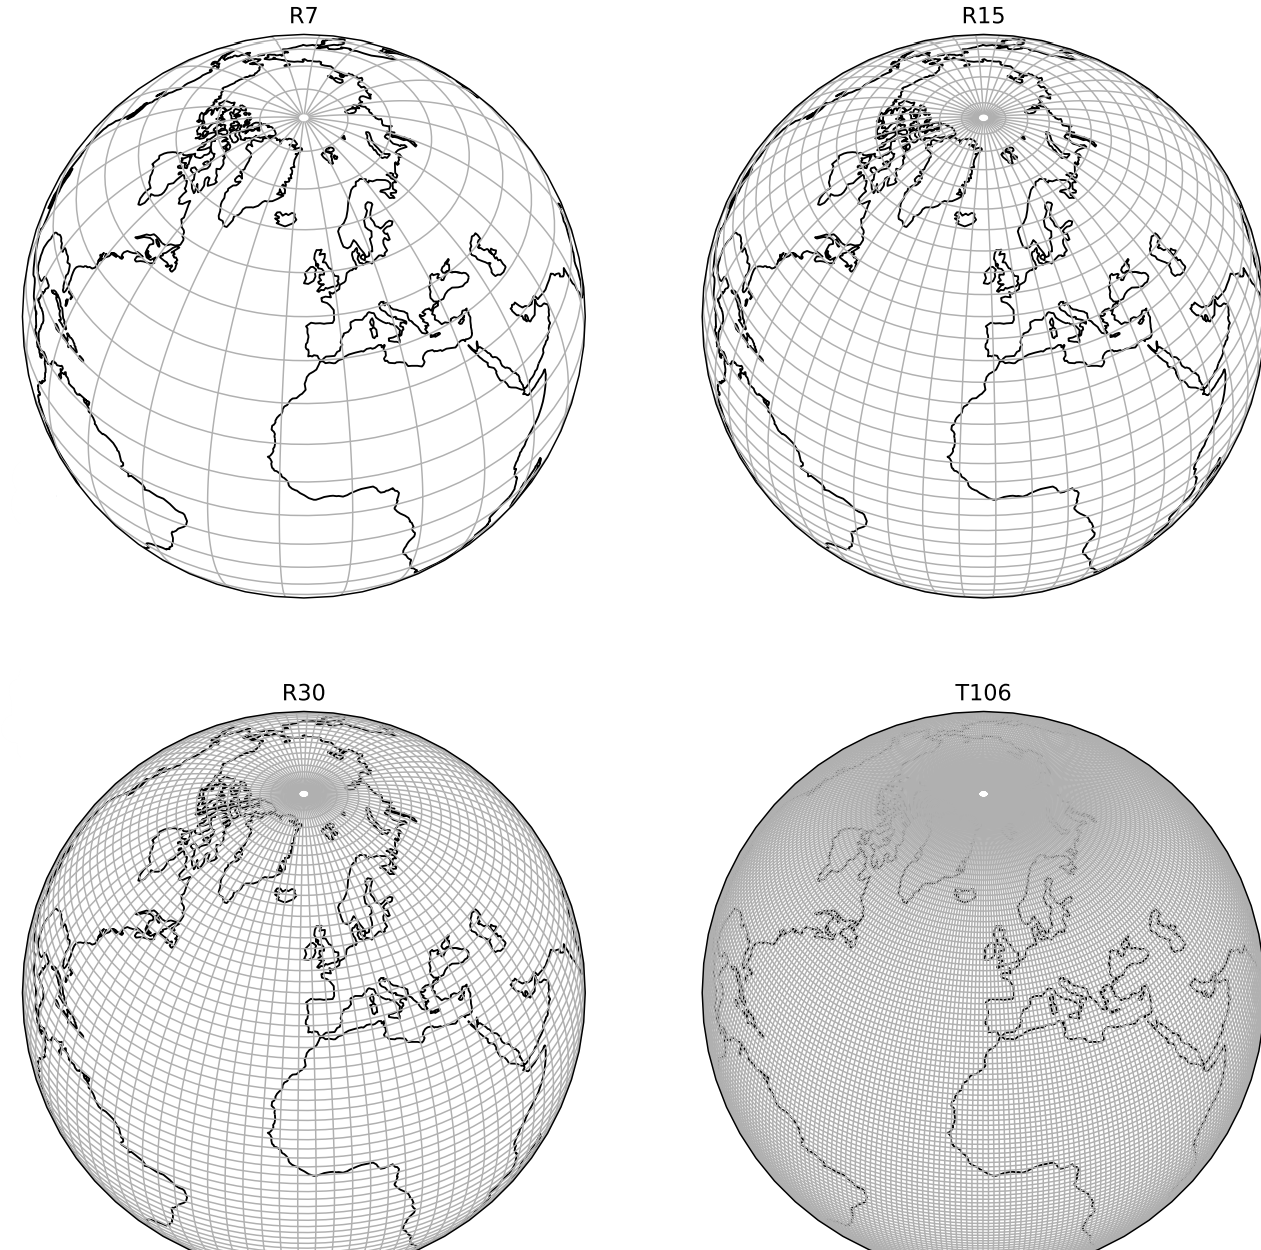
\includegraphics[width=0.5\linewidth]{uploads/gaussian grids.png}
	\caption{Examples of gaussian grids}
	\label{fig:enter-label}
\end{figure}
A Gaussian grid is a type of non-uniform grid designed to minimize numerical errors when integrating over latitude bands on a spherical surface. The key feature of a Gaussian grid is that the grid points are more concentrated at the poles (where more detailed information is often needed) and become sparser toward the equator $\rightarrow$ commonly used in spectral methods to represent variables (such as temperature or wind) in terms of spherical harmonics. The Gaussian grid is particularly useful when integrating over the Earth's spherical surface.
\subsubsection{Numerical Transform}
The discrete Fourier transform is computed numerically very efficiently by using a Fast Fouriertransform (FFT).
The integral over latitudes is a discrete Legendre transform and it requires the accurate discrete computation of the integral. It can be accomplished by a Gaussian
quadrature at $N$ special quadrature points $\mu_i$. Mathematically, the $\mu_i$ are the roots of the ordinary Legendre polynomials, which are used to compute the $N$-latitudes of the Gaussian grid between the two poles
$$\int_{-1}^1 f(x)dx\approx\displaystyle\sum_iw_if(\mu_i)$$
Gauss showed that a $N$-point \textbf{Gaussian quadrature} yields an exact result for polynomials of degree $2N-1$ or less by a suitable choice of the nodes $\mu_i$ and weights $w_i$ for $i=1,\dots,N$. Efficient algorithms have been developed to execute fast and exploit new architectures.
\begin{figure}[htpb]
	\centering
	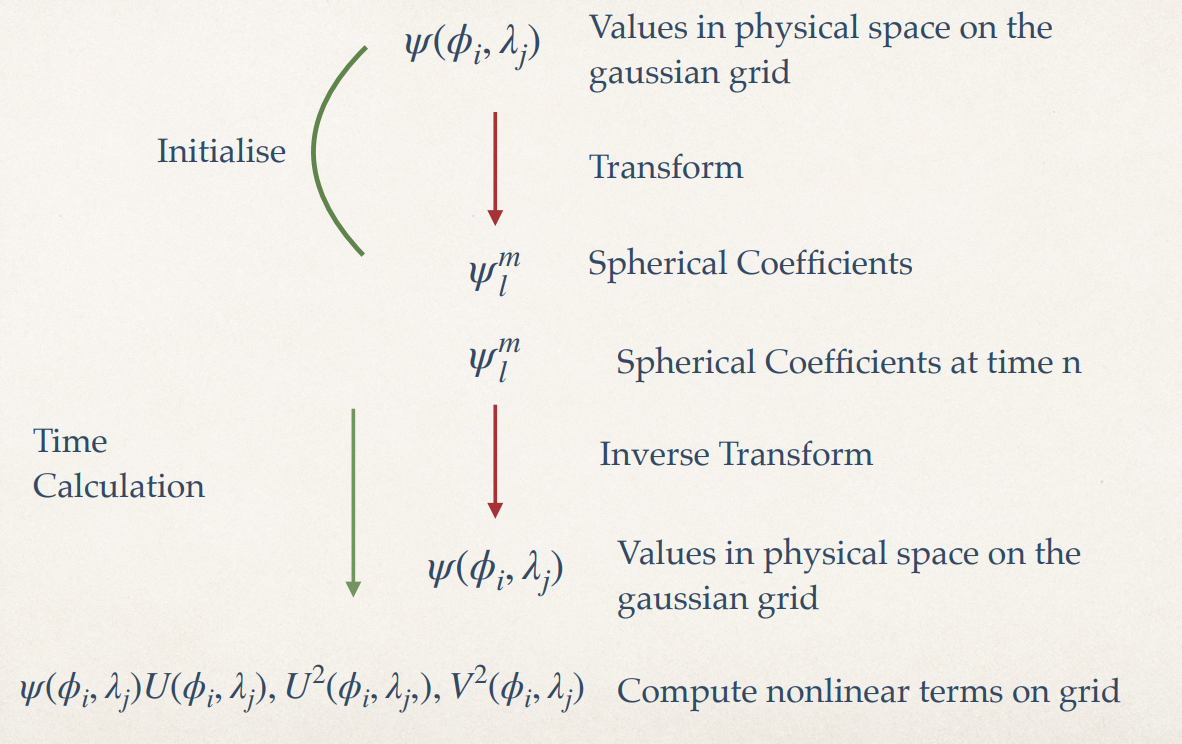
\includegraphics[width=0.5\linewidth]{uploads/Screenshot 2024-11-19 125912.png}\quad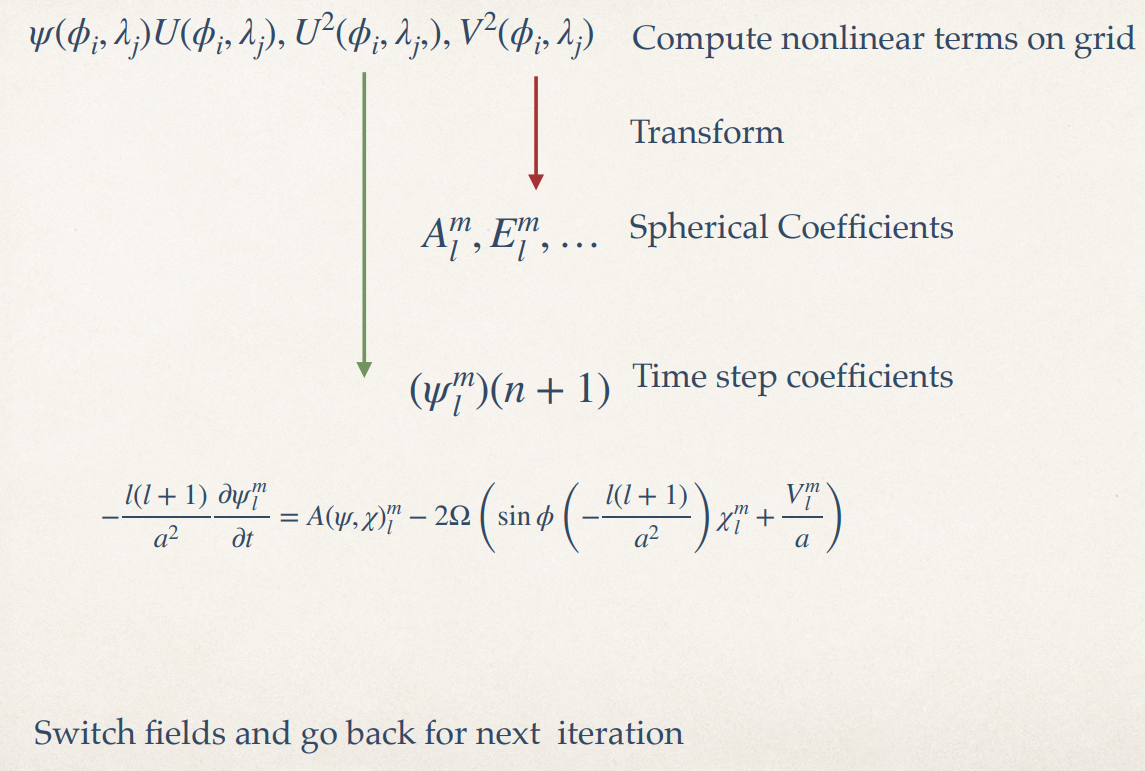
\includegraphics[width=0.5\linewidth]{uploads/Screenshot 2024-11-19 130025.png}
	\caption{The transform cycle in the time-stepping}
	\label{fig:transform cycle}
\end{figure}




\subsection{Truncation}
The very first we have to do is choose how many function to
use: the truncation order M and J. We have two indices, so
we can arrange them in a plane.

\begin{figure}[htpb]
	\centering
	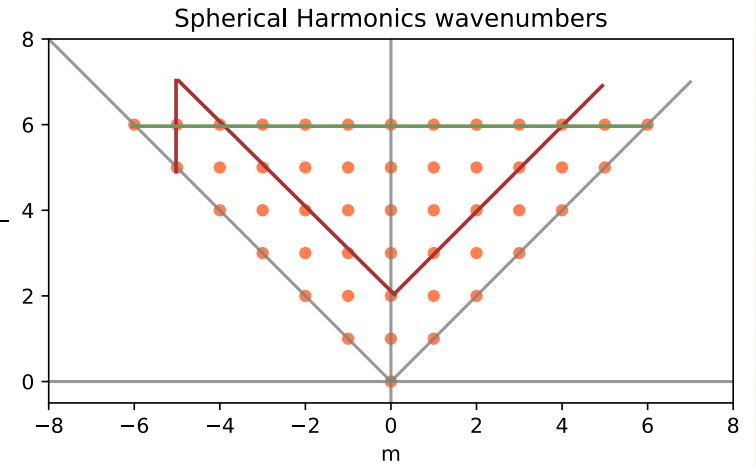
\includegraphics[width=0.5\linewidth]{uploads/Screenshot 2024-11-17 204935.png}\quad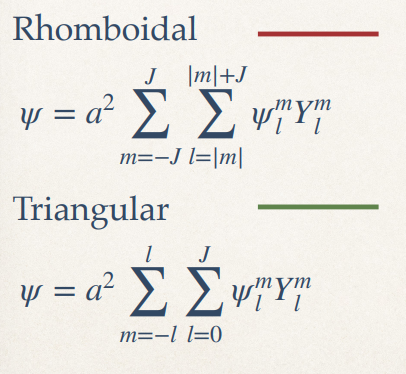
\includegraphics[width=0.25\linewidth]{uploads/Screenshot 2024-11-17 205109.png}
	\caption{a) spherical harmonics wavenumbers; b) form of the truncations}
	\label{fig:The two most used truncation}
\end{figure}

\begin{figure}[htpb]
	\centering
	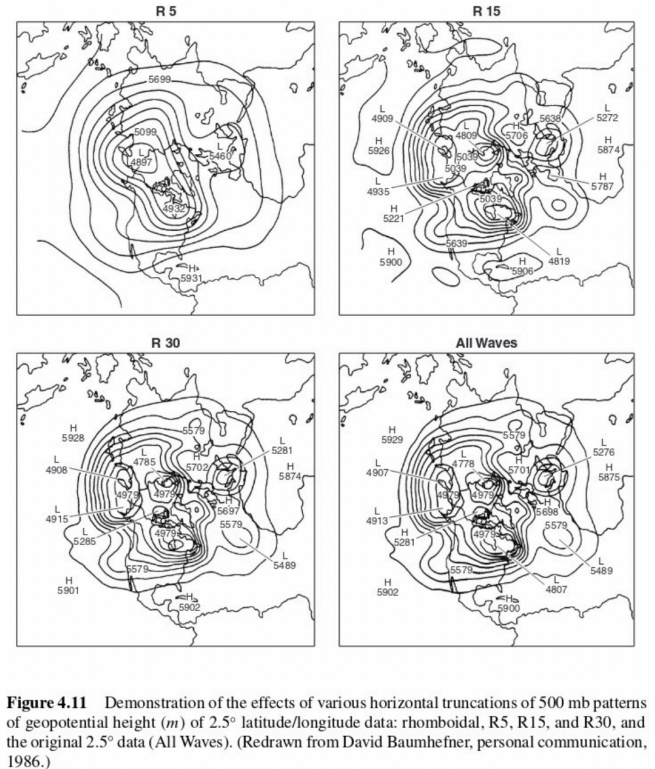
\includegraphics[width=0.4\linewidth]{uploads/Screenshot 2024-11-17 205236.png}\quad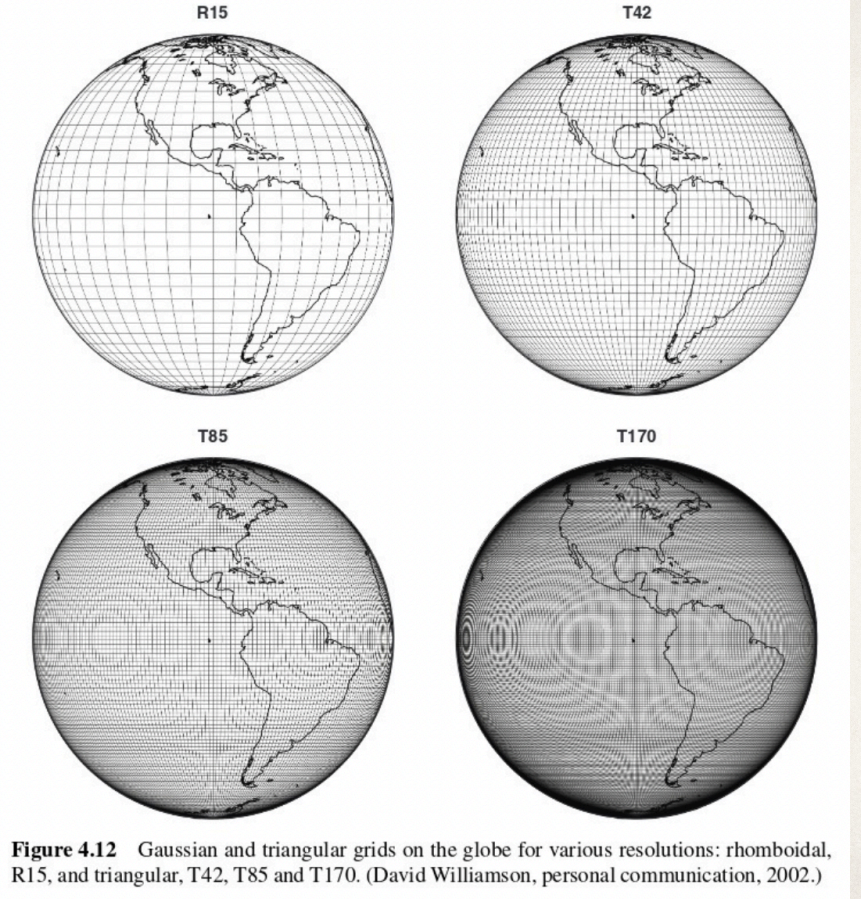
\includegraphics[width=0.4\linewidth]{uploads/Screenshot 2024-11-17 205827.png}
	\caption{Effects of truncation}
	\label{fig:enter-label}
\end{figure}
Many climate models have used a rhomboidal truncation, R, of 15 waves numbers, i.e., J=15, labeled R15. R15 gives a good approximation to the large-scale motions of the atmosphere but misses some of the smaller scale features. Increasing the resolution to R30 improves the representation to the original 2.5° data, while coarsening the resolution to R5 makes the pattern much too smooth.\\



It is not clear which type of spectral truncation is best. If triangular truncation (T) is used, then some high-frequency modes (small scales) are neglected. This truncation retains all modes where the total wave number is below a specified cutoff.  If the resolution (number of grid points or spectral modes) is high enough, the type of truncation might not matter much because the neglected modes correspond to very small scales that have minimal influence on large-scale dynamics.



\subsection{Summary}
Spectral models are a class of numerical methods used in climate system modeling to represent atmospheric, oceanic, and other geophysical phenomena. They are particularly effective for solving partial differential equations (PDEs) that describe fluid dynamics (such as the equations governing atmospheric or oceanic flow) by using mathematical functions in the form of Fourier series or spherical harmonics, rather than on a grid of points as in traditional finite difference or finite element models. \\

Spectral models represent physical variables (e.g., temperature, pressure, wind speed) as a sum of basic functions, which are typically \textit{Fourier series} (in the case of periodic domains) or \textit{spherical harmonics} (in the case of global models on a spherical surface like the Earth). This approach allows for highly accurate representations of large-scale patterns with relatively few computational elements.

\subsubsection{How to construct a spectral model}
\begin{itemize}
	\item \textcolor{RoyalBlue}{Governing Equations}: the physical equations that govern the climate system. For example, the governing equations for atmospheric dynamics are the \textit{Navier-Stokes equations} or \textit{primitive equations} (momentum, mass conservation, energy conservation).
	\item \textcolor{Sepia}{Linearization}: in many spectral models, the equations are linearized or approximated to simplify the computational process (e.g.,$\Phi=\overline{\Phi}+\Phi'$). This often involves assuming that deviations from a mean state are small and can be treated as perturbations.
	\item \textcolor{RoyalPurple}{Fourier or Spherical Harmonic Decomposition}: the physical fields are expanded in terms of a set of basis functions. For atmospheric and climate models on the Earth's surface, spherical harmonics are the most common. For a simpler system, Fourier transforms might be used for periodic domains (e.g., a wave equation on a flat domain).

	\item \textcolor{OliveGreen}{Transformation to Spectral Space}: The variables (e.g., velocity components) are expressed in terms of their spectral coefficients in the Fourier or spherical harmonic basis. The system of equations then becomes a set of equations for these coefficients, which are typically simpler to solve than the original PDEs.
\end{itemize}

\textbf{Truncation of Spectral Models}

The number of terms in the Fourier or spherical harmonic expansion is typically \textbf{finite}, and the expansion is \textbf{truncated} at a certain point to make the computation feasible. This truncation introduces a trade-off between \textit{accuracy} and \textit{computational cost}.

\begin{enumerate}
	\item \textbf{Fourier Expansion}: in a Fourier expansion, the truncation involves limiting the number of sine and cosine terms that represent the spatial variability of a field. This results in a finite spectral resolution for the model.
	\item \textbf{Spherical Harmonics Expansion}: for spherical models like global climate models, the variables (e.g., temperature, wind, pressure) are expanded in terms of \textbf{spherical harmonics} $Y_l^m(\phi,\lambda)$, which are functions defined on the surface of a sphere. These harmonics have two indices:
	      \begin{enumerate}
		      \item  $l$ is the degree,
		      \item $m$ is the known in this context as \textit{East-West planetary wavenumber}, waves around a latitudinal circle (related to the longitudinal symmetry).
	      \end{enumerate}
	      The expansion of a field $f(\phi, \lambda)$ on the sphere is: $$f(\phi, \lambda)=\displaystyle\sum_{l=0}^L\displaystyle\sum_{m=-l}^la_{lm}Y_l^m(\phi,\lambda)$$
	      where $L$ is the truncation level. The truncation level determines the maximum degree of spherical harmonics included in the model.
\end{enumerate}

\subsubsection{Helmholtz theorem}
You can decompose the velocity field into two scalar fields: the streamfunction $\psi$ and the velocity potential $\chi$, this will simplify our analysis as a  vector will transform as a vector changing its components, while a scalar will not change in different transformations. This theorem shows that you could represent a vector as function of two scalars (NB the gradient is a vector, see the Appendix\ref{app}). The vector is depending on the meridional gradient of the streamfunction and vertical of the velocity potential.


The atmospheric is almost rotational, you can take the curl of $V$ ($\nabla \times V$) that's vorticity, described as the Laplacian of $\chi$. If the potential $\chi$ is very small , then the atmosphere is dominated by the the streamfunction $\psi$. This describes very well the atmospheric circulation outside of the tropics, there $\chi$ becomes significant.
\subsubsection{Spherical Harmonics}
Spherical harmonics are mathematical functions defined on the surface of a sphere. They are particularly useful in climate modeling because the Earth is roughly spherical, and they naturally represent the angular components of a field. More details can be found in \ref{app}.

\begin{itemize}
	\item \textbf{Mathematical Form}: Spherical harmonics $Y_l^m(\phi,\lambda)$ are solutions to the Laplace equation in spherical coordinates. They depend on two variables:
	      \begin{itemize}
		      \item $\phi$ (latitude, ranging from $0°$ to $180°$),
		      \item $\lambda$ (longitude, ranging from $0°$ to $360°$).
	      \end{itemize}The functions are orthogonal, meaning that integrals of different harmonic modes are zero unless they are the same mode (or its conjugate).
	\item \textbf{Properties}:
	      \begin{itemize}
		      \item The spherical harmonic functions form a complete, orthogonal set on the sphere, making them ideal for representing global fields like temperature, pressure, and wind patterns.
		      \item The index $l$ controls the \textbf{spatial scale} of the variations, with higher values of $l$ corresponding to finer (smaller-scale) features, $l\geq|m|$.
		      \item The index $m$ corresponds to the \textbf{longitudinal symmetry} of the pattern. For a given $l$, there are $2l+1$ different $m$-values, ranging from $-l$ to $+l$.
	      \end{itemize}
	\item \textbf{Truncation}: in spectral models, the expansion is truncated at a maximum value of $J$ in our discussion. The number of coefficients increases rapidly as $J$ increases because the number of distinct $m$-values for each $l$ is $2l+1$. For example, the total number of coefficients for a given truncation level $J$ is given by:
	      $$N_{\text{coeff}}=\displaystyle\sum_{l=0}^J(2l+1)$$
	      which grows roughly as $J^2$. Truncating at a high $J$ allows the model to capture finer details, but increases computational cost.
	      \textsc{Example}: For a truncation level $J=10$, you would include all spherical harmonics up to degree 10. The number of coefficients would be:$$N_{\text{coeff}}=\displaystyle\sum_{l=0}^{10}(2l+1)=1+3+5+7+9+11+13+15+17+19+21=100$$
	      These coefficients are used to represent the field in terms of spherical harmonics.
\end{itemize}

\subsubsection{Advantages and Challenges of Spectral Methods}

\paragraph{Advantages}
Accuracy with fewer points: spectral methods can represent large-scale features of the climate system (such as planetary waves, jet streams, etc.) very accurately with relatively few degrees of freedom (i.e., fewer spectral coefficients) compared to grid-based models $\rightarrow$ accuracy with fewer points. Also, for certain types of problems, spectral methods can be more efficient than finite difference methods because they avoid the need for fine grids over the entire domain $\rightarrow$ efficient computation.
\paragraph{Challenges}
\begin{itemize}
	\item \textbf{Nonlinearity}: Spectral models can become more challenging when dealing with highly nonlinear phenomena (e.g., turbulence or convection). The nonlinear terms in the equations can introduce additional complexity, requiring special treatment like non-linear spectral operators.
	\item \textbf{Gridpoint-based variables}: While spectral methods work well for smooth solutions, they can struggle with sharp gradients or discontinuities, which are more naturally handled by grid-based methods.
	\item \textbf{Computational cost}: As the truncation level increases, the number of terms in the expansion grows quickly, increasing the computational cost. The choice of truncation level is often a balance between accuracy and available computational resources.
\end{itemize}



\section{Lagrangian Methods}
Remember the Gibbs phenomenon: the Fourier transform (Fourier series but with non-periodic functions with continuous range of frequencies) had problems in
transforming functions with jumps.
The Fourier transform of a function with a discontinuity produces a frequency spectrum that decays slowly, creating a high-frequency ringing in the reconstructed signal (when using an inverse Fourier transform).
This ringing is analogous to the overshoot in Fourier series. It occurs because truncating the Fourier transform (e.g., ignoring very high frequencies) is equivalent to applying a low-pass filter, which introduces oscillations due to sharp edges in the signal.


This is a property not only of the
Fourier transform but the all orthogonal transforms so the Legendre
transform in the latitudinal direction will suffer from the same issue. This
is a problem with any spectral model that will have difficulty in
representing gradients steeper then the grid can sustain.
Mountains will pose a problem, but also positive-definite quantities like
water vapor and chemical tracers.

\begin{figure}[h!]
	\centering
	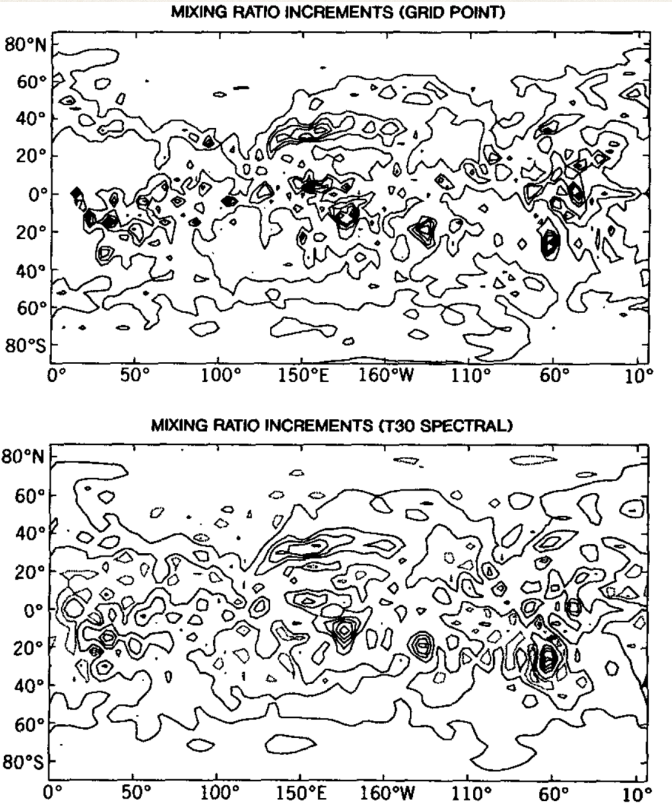
\includegraphics[width=0.5\linewidth]{uploads/Screenshot 2024-11-19 130213.png}
	\caption{Lagrangian Methods}
	\label{fig:lag method}
\end{figure}
In an Eulerian advection scheme an observer watches the world evolve around her at a fixed geographical point. Such schemes work well on regular Cartesian meshes (facilitating vectorization and parallelization of the resulting code), but often lead to overly restictive time steps due to considerations of computational stability. In a Lagrangian advection scheme an observer watches the world evolve around him as he travels with fluid particle. Such schemes can often use much larger time steps than Eulerian ones, but have the disadvantage that an initially regularly spaced set of particles will generally evolve to a highly irregularity spaced set at later times, and important features of the flow may consequently not be well represented. The idea behind semi-Lagrangian advection schemes is to try to get the best of both worlds: the regular resolution of Eulerian schemes and the enhanced stability of Lagrangian ones. This is achieved by using a different set of particles at each time step the set of particles being chosen such that they arrive exactly at the points of a regular Cartesian mesh at the end of the time step.

\subsection{Semi-Lagrangian Methods}
\begin{figure}[h!]
	\centering
	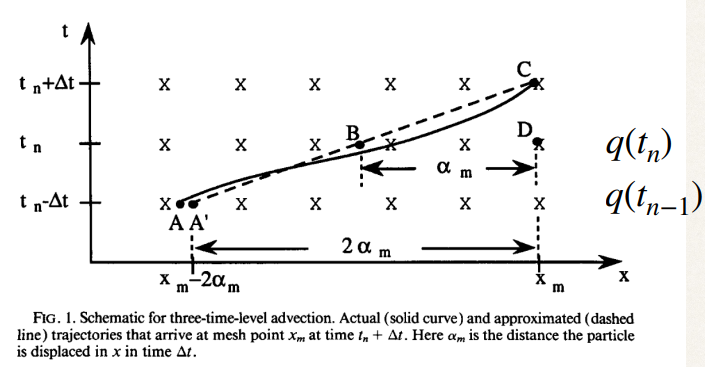
\includegraphics[width=0.5\linewidth]{uploads/Screenshot 2024-11-19 142400.png}
	\caption{Semi-Lagrangian method}
	\label{fig:enter-label}
\end{figure}
Considering:
$$\frac{dq}{dt}=\frac{\partial q}{\partial t}+U\frac{\partial q}{\partial x}=S(x,t)$$
with $\frac{dx}{dt}=U(x,t)$
Integrating along the trajectory $A'C$:
$$q(x_m,t_n+\Delta t)=q(x_m-2\alpha_m,t_n-\Delta t)+2\Delta tS(x-\alpha_m,t_n)$$
Assuming it is started at $-2\alpha m$ , and because it was transported by $(t_n - \Delta t)$, the $S$ (source or sink term for $q$, where $q$ will change along a trajectory only as a function of $S$) is computed at $t_n$ so at $\alpha_m$ the displacement can be found solving:
$$\alpha_m=\Delta tU(x-\alpha_m,t_n)$$
and considering:
$$q(x-2\alpha_m,t-\Delta t)$$ this quantity may not be at the grid point, I have to interpolate. This is preserving the trace and allowing me to look at a long time step. This transported quantities are used in a passive way because it doesn't reflect immediately in the rest of the dynamic.
\begin{wrapfigure}{r}{0.58\textwidth}
	\begin{center}
		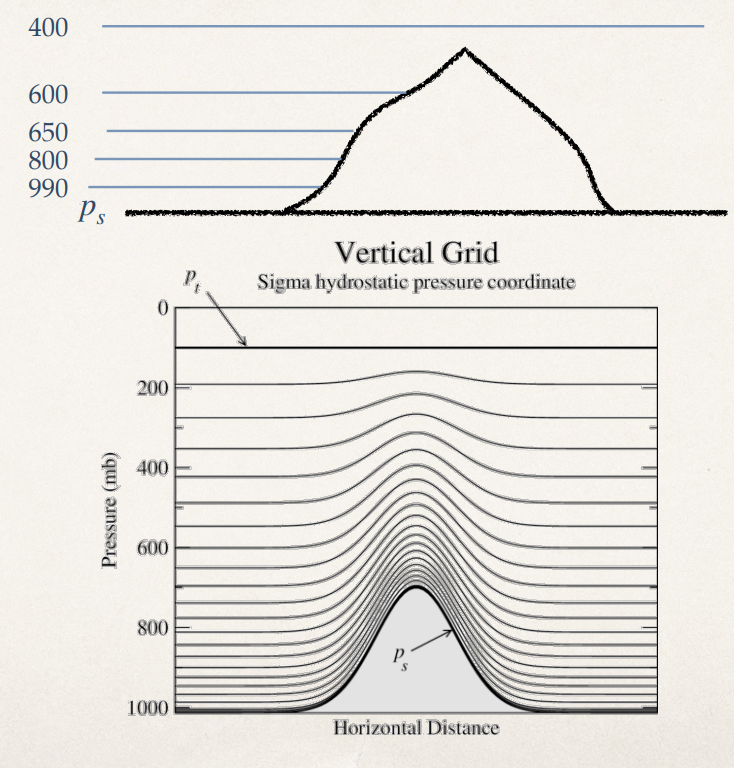
\includegraphics[width=0.45\linewidth]{uploads/Screenshot 2024-11-19 143432.png}
	\end{center}
	\caption{Pressure coordinates vs sigma coordinates}
	\label{fig:sigmababy}
\end{wrapfigure}
\section{Vertical coordinates}
The original vertical coordinate was the Z coordinate that is simply the
geometric height. However, as the atmosphere is in hydrostatic balance, one could use the pressure as a vertical coordinate.
$$(\lambda, \phi, z)\rightarrow(u,v,w) $$
$$(\lambda, \phi, p)\rightarrow (u,v,\dot{p}=\omega)$$
as $$\vec{\nabla}\cdot\vec{v}+\frac{\partial\omega}{\partial p}=0$$
This implies to consider more layers in the vertical, each of these with different coefficients, then discretizing in the surface (in the making of models).
However, spectral models require to have integrals over spheres: what happens if there are mountains? There will be boundary conditions.
This choice hence as the problem that the surface pressure intersects the surface especially over mountains creating problems numerically in the definition of the boundary condition.

Phillips (1957) proposed to use a normalised pressure coordinate, $$\sigma=\frac{p}{p_s}$$ The vertical velocity is now $\dot{\sigma}$. The spectral expansion might lead to bumps that propagate all the way up, they will create errors in the pressure gradient force. To have smoother bumps: another coordinate is introduced as in the figure \ref{fig:sigmababy}. As the grid is staggered also in the vertical, in this way we'll get half layers: NB gound level is always an half-level.
\paragraph{Hybrid coordinates}
It is a sigma coordinates close to the ground, but smoothly transform into a
pressure coordinate far from the ground $$\sigma=\frac{p-p_T}{p_S-p_T}$$
